\documentclass[a4paper,12pt,twoside]{memoir}

% Castellano
\usepackage[spanish,es-tabla]{babel}
\selectlanguage{spanish}
\usepackage[utf8]{inputenc}
\usepackage[T1]{fontenc}
\usepackage{lmodern} % Scalable font
\usepackage{microtype}
\usepackage{placeins}

\RequirePackage{booktabs}
\RequirePackage[table]{xcolor}
\RequirePackage{xtab}
\RequirePackage{multirow}

% Links
\PassOptionsToPackage{hyphens}{url}\usepackage[colorlinks]{hyperref}
\hypersetup{
	allcolors = {red}
}

% Ecuaciones
\usepackage{amsmath}

% Rutas de fichero / paquete
\newcommand{\ruta}[1]{{\sffamily #1}}

% Párrafos
\nonzeroparskip

% Huérfanas y viudas
\widowpenalty100000
\clubpenalty100000

\let\tmp\oddsidemargin
\let\oddsidemargin\evensidemargin
\let\evensidemargin\tmp
\reversemarginpar

% Imágenes
% Comando para insertar una imagen en un lugar concreto.
% Los parámetros son:
% 1 --> Ruta absoluta/relativa de la figura
% 2 --> Texto a pie de figura
% 3 --> Tamaño en tanto por uno relativo al ancho de página
\usepackage{graphicx}

\usepackage[sorting=none]{biblatex}
\addbibresource{bibliografia.bib}
\usepackage{rotating}
\newcommand{\imagen}[3]{
	\begin{figure}[!h]
		\centering
		\includegraphics[width=#3\textwidth]{#1}
		\caption{#2}\label{fig:#1}
	\end{figure}
	\FloatBarrier
}







\graphicspath{ {./img/} }

% Capítulos
\chapterstyle{bianchi}
\newcommand{\capitulo}[2]{
	\setcounter{chapter}{#1}
	\setcounter{section}{0}
	\setcounter{figure}{0}
	\setcounter{table}{0}
	\chapter*{#2}
	\addcontentsline{toc}{chapter}{#2}
	\markboth{#2}{#2}
}

% Apéndices
\renewcommand{\appendixname}{Apéndice}
\renewcommand*\cftappendixname{\appendixname}

\newcommand{\apendice}[1]{
	%\renewcommand{\thechapter}{A}
	\chapter{#1}
}

\renewcommand*\cftappendixname{\appendixname\ }

% Formato de portada

\makeatletter
\usepackage{xcolor}
\newcommand{\tutor}[1]{\def\@tutor{#1}}


\newcommand{\course}[1]{\def\@course{#1}}
\definecolor{cpardoBox}{HTML}{E6E6FF}
\def\maketitle{
  \null
  \thispagestyle{empty}
  % Cabecera ----------------
\begin{center}
  \noindent
\includegraphics[width=\textwidth]{cabeceraSalud}\vspace{1.5cm}%
\end{center}
  
  % Título proyecto y escudo salud ----------------
  \begin{center}
    \begin{minipage}[c][1.5cm][c]{.20\textwidth}
        
\includegraphics[width=\textwidth]{escudoSalud.pdf}
    \end{minipage}
  \end{center}
  
  \begin{center}
    \colorbox{cpardoBox}{%
        \begin{minipage}{.8\textwidth}
          \vspace{.5cm}\Large
          \begin{center}
          \textbf{TFG del Grado en Ingeniería de la Salud}\vspace{.6cm}\\
          \textbf{\LARGE\@title{}}
          \end{center}
          \vspace{.2cm}
        \end{minipage}
    }%
  \end{center}
  
    % Datos de alumno, curso y tutores ------------------
  \begin{center}%
  {%
    \noindent\LARGE
    Presentado por \@author{}\\ 
    en Universidad de Burgos\\
    \vspace{0.5cm}
    \noindent\Large
    \@date{}\\
    \vspace{0.5cm}
    %Tutor: \@tutor{}\\ % comenta el que no corresponda
    Tutor: \@tutor{}\\
  }%
  \end{center}%
  \null
  \cleardoublepage
  }
\makeatother

\newcommand{\nombre}{Carmen Marcos Gordillo}
\newcommand{\nombreTutor}{Guirguis Zaki Guirguis Abdelmessih} 
\newcommand{\dni}{71756805W} 

% Datos de portada
\title{Solución tecnológica para la monitorización de síntomas motores en pacientes con Párkinson}
\author{\nombre}
\tutor{\nombreTutor}
\date{\today}


\begin{document}

\maketitle


\newpage\null\thispagestyle{empty}\newpage

%%%%%%%%%%%%%%%%%%%%%%%%%%%%%%%%%%%%%%%%%%%%%%%%%%%%%%%%%%%%%%%%%%%%%%%%%%%%%%%%%%%%%%%%
\thispagestyle{empty}


\noindent
\includegraphics[width=\textwidth]{cabeceraSalud}\vspace{1cm}

\noindent D. \nombreTutor, profesor del departamento de Ingeniería Electromecánica, área de Tecnología electrónica.

\noindent Expone:

\noindent Que el alumno D. \nombre, con DNI \dni, ha realizado el Trabajo final de Grado en Ingeniería de la Salud titulado título del trabajo. 

\noindent Y que dicho trabajo ha sido realizado por el alumno bajo la dirección del que suscribe, en virtud de lo cual se autoriza su presentación y defensa.

\begin{center} %\large
En Burgos, {\large \today}
\end{center}

\vfill\vfill\vfill

% Author and supervisor
\begin{minipage}{0.45\textwidth}
\begin{flushleft} %\large
Vº. Bº. del Tutor:\\[2cm]
D. \nombreTutor
\end{flushleft}
\end{minipage}
\hfill
\begin{minipage}{0.45\textwidth}

\end{minipage}
\hfill

\vfill

% para casos con solo un tutor comentar lo anterior
% y descomentar lo siguiente
%Vº. Bº. del Tutor:\\[2cm]
%D. nombre tutor


\newpage\null\thispagestyle{empty}\newpage




\frontmatter

% Abstract en castellano
\renewcommand*\abstractname{Resumen}
\begin{abstract}
La enfermedad de Párkinson representa el trastorno neurodegenerativo del movimiento más común, presentando en Europa una prevalencia de 108-257 casos por cada 100 000 habitantes. Los pacientes de Párkinson presentan frecuentemente como síntoma bloqueos musculares que derivan en congelación de la marcha.

El presente proyecto utiliza como punto de partida el prototipo obtenido en 2 proyectos anteriores \cite{Gonzalez2023} \cite{Martos2024}, los cuales estaban centrados en el desarrollo de una solución tecnológica hardware/software que utiliza componentes Arduino y una aplicación web para la monitorización de este síntoma. 

Se desarrollan diversas funcionalidades relativas a la aplicación web y al script Arduino del sensor: personalización de la detección de congelación de la marcha por parte del sensor, generación de gráficas e informes a partir de las actividades registradas y registro diario de fluctuaciones motoras, cuyos datos se analizan conjuntamente con las actividades para mostrar los efectos de las medicaciones en los síntomas motores del paciente. Esto aporta un feedback al profesional que sirve como ayuda a la hora de evaluar la progresión de la enfermedad y ajustar la pauta de medicaciones según los síntomas del paciente.

Se rediseña también el hardware con el objetivo de aportar al usuario una mayor comodidad y una función de reacción a la detección de congelación de la marcha.

\end{abstract}

\renewcommand*\abstractname{Descriptores}
\begin{abstract}
Enfermedad de Párkinson, congelación de la marcha, bloqueo muscular, Arduino, aplicación web, diario de fluctuaciones motoras, informe de actividades, solución tecnológica.
\end{abstract}

\clearpage

% Abstract en inglés
\renewcommand*\abstractname{Abstract}
\begin{abstract}
Parkinson's disease represents the most common neurodegenerative movement disorder, with a prevalence of 108-257 cases per 100,000 inhabitants in Europe. Parkinson's patients frequently present muscle blockages as a symptom that leads to freezing of gait.

This project uses as a starting point the prototype obtained in 2 previous projects \cite{Gonzalez2023} \cite{Martos2024}, which focused on the development of a hardware/software technological solution that uses Arduino components and a web application to monitor this symptom.

Various functionalities are developed related to the web application and the Arduino script of the sensor: customization of the detection of freezing of gait by the sensor, generation of graphs and reports from the recorded activities and daily recording of motor fluctuations, whose data is analyzed together with the activities to show the effects of the medications on the patient's motor symptoms. This provides feedback to the professional that helps when evaluating the progression of the disease and adjusting the medication regimen according to the patient's symptoms.

The hardware is also redesigned with the aim of providing the user with greater comfort and a reaction function to the detection of freezing of movement.
\end{abstract}

\renewcommand*\abstractname{Keywords}
\begin{abstract}
Parkinson's Disease, freezing of gait, muscle block, Arduino, web application, diary of motor fluctuations, activity report, technological solution.
\end{abstract}

\clearpage

% Indices
\tableofcontents

\clearpage

\listoffigures

\clearpage

\listoftables
\clearpage


\mainmatter
\capitulo{1}{Introducción}


La enfermedad de Párkinson es el segundo trastorno neurodegenerativo más común, cuyo efecto fisiológico principal es la pérdida progresiva de neuronas dopaminérgicas en la sustancia negra del cerebro. Los síntomas más comunes causados por esta disminución de dopamina son temblores, rigidez muscular y bradicinesia (lentitud en los movimientos). Estos síntomas motores en ocasiones se traducen en bloqueos de la marcha, los cuales pueden alterarla, suponer un cese total de la misma u ocasionar caídas. La monitorización continuada de los síntomas motores del Párkinson es crucial para la correcta adaptación del tratamiento a la evolución de la enfermedad por parte de los profesionales sanitarios, garantizando una mejor calidad de vida de los pacientes.

Este Trabajo de Fin de Grado (TFG) se centra en la monitorización de los bloqueos de la marcha que desembocan en un cese total de la misma. Esto se logra mediante el uso de un dispositivo hardware con componentes Arduino que registra dichos bloqueos, proporcionando también una ayuda visual para su superación, y una aplicación web de sencillo manejo destinada a la utilización por parte del paciente y el profesional sanitario. 

Esta solución tecnológica evoluciona a partir del diseño de hardware Arduino y aplicación web propuestos en los TFGs \cite{Gonzalez2023} \cite{Martos2024}, agregando mejoras en el hardware y software para una ampliación de sus funciones. Se incluye en la aplicación web la posibilidad de generar gráficas e informes, así como personalizar el tiempo de cese de la marcha necesario para que el sensor detecte un bloqueo muscular con congelamiento de la marcha mediante una sencilla prueba. Se incluyen también 2 diarios del paciente (de tomas de medicaciones y fluctuaciones motoras, los cuales al contrastarse con las actividades registradas proveen información sobre el efecto de las medicaciones en los sintomas motores del paciente. Se agrega una respuesta a la detección de bloqueos, proyectando una línea láser en el suelo para ayudar al paciente a recuperar la marcha de forma más sencilla.

En el presente documento se presenta la memoria del proyecto, comenzando por una descripción de los objetivos propuestos, una serie de conceptos teóricos relevantes para comprender el contexto de la presente solución y las tecnologías actuales en su misma línea, un apartado que describe la metodología utilizada y una descripción de los resultados obtenidos, conclusiones y líneas futuras para la mejora del proyecto.

Se incluirán adicionalmente los siguientes anexos: Anexo A, referido a la planificación temporal del desarrollo del proyecto; Anexo B, detallando un manual de usuario; Anexo C, constituyendo un manual del programador; Anexo D, con especificaciones sobre los datos con los que se trabaja durante el proyecto; Anexo E, detallando el diseño del hardware y software mediante planos y diagramas; Anexo F, sobre la especificación de requisitos; Anexo G, explicando un desarrollo experimental y anexo H, representando un anexo de sostenibilidad curricular.

Los documentos mencionados, así como los archivos de código y demás archivos relevantes se encuentran organizados en carpetas dentro del repositorio \href{https://github.com/cmg1015/TFG_Seguimiento_Parkinson}{GitHub}, en el link '\url{https://github.com/cmg1015/TFG_Seguimiento_Parkinson}'.





\capitulo{2}{Objetivos}
Este proyecto busca desarrollar una solución tecnológica hadware/software para el monitoreo de actividades y fluctuaciones motoras en pacientes con párkinson, consistente en un cinturón con una placa y otros módulos Arduino conectado a una tobillera con un sensor giroscopio/acelerómetro y una aplicación web. \\ \\
Mediante la comunicación bidireccional constante entre el hardware Arduino y el backend de la aplicación web se consigue registrar en tiempo real las actividades realizadas con su correspondiente fecha y hora, así como la reacción en tiempo real a los bloqueos detectados, contribuyendo a la reanudación de la marcha mediante la proyección de una línea láser en el suelo.\\ \\
La utilización regular de la aplicación web y el dispositivo permite obtener y analizar información relativa a la toma de medicaciones, fluctuaciones ON/OFF detectadas por el paciente y las actividades realizadas. El análisis de este conjunto de información supone una herramienta útil para la evaluación del progreso de la enfermedad y del tratamiento actual.
\subsection{Objetivos principales}
\begin{enumerate}
    \item Diseñar y construir un prototipo hardware consistente en un cinturón y una tobillera, que resulte cómodo y de bajo coste y que reaccione al detectar una congelación de la marcha mediante una proyección de línea láser en el suelo.
    \item Implementar funcionalidades software para la personalización del funcionamiento del hardware desde la aplicación web y el registro de tomas de medicación y sintomatología diario, el cual será analizado para obtener datos relevantes sobre la evolución de la enfermedad y la efectividad del tratamiento.
\end{enumerate}

\subsection{Objetivos de hardware}
\begin{enumerate}
    \item Diseñar un prototipo que, contando con todos los módulos descritos en el trabajo de fin de grado \cite{Martos2024}, resulte flexible y pueda colocarse en un cinturón con compartimentos para una mayor comodidad del usuario. 
    \item Añadir un componente de módulo láser, que proyecte una línea en el suelo al detectar un bloqueo muscular con cese de la marcha para ayudar al paciente a reanudarla.
    \item Agregar un componente RTC, con el objetivo de registrar la fecha y hora de realización de las actividades.
\end{enumerate}

\subsection{Objetivos de desarrollo software}
\subsubsection{Funciones de la aplicación web}
\begin{enumerate}
    \item Agregar una prueba de personalización, que permita registrar una actividad con ciertas particularidades: se omitirá la detección de bloqueos y se permitirá la finalización y guardado de resultados tan sólo si se han superado los 10 pasos. Esta prueba se utilizará para registrar el tiempo medio que tarda el paciente en dar un paso, y a partir de ello determinar el número de segundos en reposo que debe detectar el sensor para detectar un bloqueo muscular con cese de la marcha. 
    Estas pruebas se guardarán en una tabla separada de la base de datos y el número de segundos determinado será enviado al hardware, que funcionará acorde al mismo desde ese momento en adelante.
    \item Como nueva funcionalidad del tipo de usuario 'profesional', se podrá agregar una pauta de medicación determinada a cada paciente.
    \item Como nueva funcionalidad del tipo de usuario 'paciente' se incluye la posibilidad de registrar un diario, en el que se registrarán las tomas de medicación y los estados ON/OFF del paciente. Al resultar normalmente repetitivas las tomas de medicación diarias, se establecerán como respuestas predeterminadas al formulario la pauta de medicación que el profesional haya asignado al paciente.
\end{enumerate}
\subsubsection{Funciones del código Arduino}
\begin{enumerate}
    \item Manejar de forma adecuada el encendido y apagado del módulo láser tras la detección de cese de la marcha.
    \item Manejo del módulo RTC, almacenando junto con la información de la actividad (bloqueos, tiempo, pasos...) la fecha y hora en la que ha sido realizada, y enviando dichos valores de forma adecuada a los archivos de código correspondientes al backend de la aplicación web.
    \item Flexibilizar la detección de bloqueos, cambiando el número fijo de segundos de reposo del sensor a partir de los cuales se detecta un cese de la marcha (5 segundos) por un número variable entre 1 y 20 segundos, en función de la información recibida desde la app.
\end{enumerate}
%Objetivos principales del trabajo realizado.


%Este apartado explica de forma precisa y concisa cuales son los objetivos que se persiguen con la realización del proyecto. Se puede distinguir entre:
%\begin{enumerate}
 %   \item Los objetivos marcados por los requisitos del software/hardware/análisis a desarrollar.
  %  \item Los objetivos de carácter técnico, relativos a la calidad de los resultados, velocidad de ejecución, fiabilidad o similares.
   % \item Los objetivos de aprendizaje, relativos a aprender técnicas o herramientas de interés. 
%\end{enumerate}









\capitulo{3}{Conceptos teóricos}

\section{Conceptos teóricos básicos}

\subsection{Enfermedad de Párkinson}
La enfermedad de Párkinson es un trastorno neurodegenerativo del sistema nervioso central caracterizado por la pérdida de neuronas dopaminérgicas en los ganglios basales (sustancia negra), derivando en una deficiencia de dopamina que afecta a la regulación de las estructuras cerebrales implicadas en el control del movimiento. \\ \\
Se trata del trastorno neurodegenerativo muscular más común, con unos ratios de incidencia de 11–19/100 000 casos y de prevalencia de 108–257/100 000 casos al año en Europa. \cite{balestrino2020parkinson}

\subsubsection{Causas}
Las causas de la enfermedad de Párkinson no han sido claramente establecidas. Sin embargo, hay un creciente consenso sobre la convergencia de ciertos mecanismos autónomos celulares y mecanismos no autónomos celulares como causas del deterioro de las neuronas dopaminérgicas\cite{hirsch2013pathogenesis}:
\begin{itemize}
    \item Mecanismos autónomos celulares: La regulación por el coactivador transcripcional PGC-1 alfa se encuentra alterada en pacientes con gen parkin no funcional. Esta regulación es esencial para la biogénesis mitocondrial, el metabolismo de especies reactivas del oxígeno (ROS) y la respiración celular.\\
    La sobreexpresión de proteína PARIS causada por la inactivación del gen parkin  reprime la expresión del coactivador transcripcional PGC-1 alfa, impidiendo la activación de NRF-1 (factor respiratorio nuclear 1), el cual es clave en la respiración mitocondrial. \cite{SHIN2011689}
    \item Mecanismos no autónomos celulares: La agregación anormal de proteínas, en particular de la  alfa-sinucleína (alfa-syn) causa degeneración neuronal en la sustancia negra y en el cuerpo estriado. \\
    La alfa-syn es una proteína presente en los terminales presinápticos de las neuronas, la cual resulta esencial para el correcto funcionamiento mitocondrial.  La acumulación de oligómeros y agregados más grandes de alfa-syn mal plegada, debido a factores genéticos o ambientales, se propaga en pacientes con párkinson a lo largo de las distintas etapas de la enfermedad mediante un mecanismo similar al de los priones, llegando a afectar numerosas áreas como el bulbo olfatorio, el cortex cerebral o la amígdala y produciendo diferente sintomatología en el paciente según las áreas afectadas. \cite{10.3389/fnins.2019.00552}
\end{itemize}
La acumulación de mitocondrias disfuncionales causada por una deficiente función de parkin y PINK1 (que eliminarían mitocondrias disfuncionales en condiciones normales) resulta en una pérdida de función de neuronas dopaminérgicas de la sustancia negra, derivando en una progresiva pérdida de funciones cerebrales. \cite{hirsch2013pathogenesis}
\subsubsection{Diagnóstico y sintomatología}
El primer paso hacia un diagnóstico de párkinson es la detección de parkinsonismo, basándose este término en 3 manifestaciones motoras cardinales, las cuales deben aparecer claramente y sin otra causa definida\cite{postuma2015mds}: 
\begin{itemize}
    \item Bradicinesia: ralentización de los movimientos y disminución de su amplitud. Debe estar presente combinada con al menos una de las siguientes manifestaciones.
    \item Temblores en reposo
    \item Rigidez
\end{itemize}
La Sociedad de Trastornos del movimiento (MDS) establece una guía para diagnosticar parkinson de forma clínica o una probabilidad de párkinson. Para ello describe 
una serie de criterios de exclusión, criterios de apoyo y banderas rojas.\cite{postuma2015mds}

\subsubsection{Tratamiento de los síntomas motores}
Existen numerosas formas de tratar los síntomas motores en pacientes con párkinson. La elección en el tratamiento farmacológico del paciente dependerá en gran medida de la edad y el compromiso funcional que presentan los pacientes. Algunos de los tratamientos farmacológicos utilizados para tratar la sintomatología motora son \cite{marin2018enfermedad}:
\begin{itemize}
    \item Levodopa: Fármaco precursor de la dopamina, el cual se transforma en esta sustancia tras la acción de la enzima dopa-descarboxilasa. Para asegurar el paso a través de la barrera hematoencefálica previo a esta reacción se utiliza conjuntamente con inhibidores de la enzima dopa-descaroxilasa periférica, como la carbidopa y la benserazida. \\
    Es el fármaco más utilizado para el tratamiento de los síntomas motores de la enfermedad de Párkinson, debido a su efectividad en la reducción de temblores, bradicinesia y rigidez. Sin embargo, la toma a largo plazo durante 5-10 años produce complicaciones en más de la mitad de los pacientes, por lo cual su administración suele intentar evitarse en los pacientes más jóvenes.
    \item Agonistas dopaminérgicos: Medicamentos que estimulan los receptores de dopamina, aumentando de esta forma los efectos de esta sustancia en los pacientes sin aumentar la concentración de la misma. Producen menos fluctuaciones motoras y discinesias en comparación con la levodopa. Sin embargo, su eficacia se reduce conforme avanza la enfermedad, siendo necesario en estas etapas el acompañamiento de fármacos como la levodopa para poder manejar los crecientes síntomas.
    \item Inhibidores de la monoaminooxidasa tipo B (iMAO-B): Medicamentos como la selegilina, rasagilina y safinamida inhiben la enzima MAO-B, encargada de descomponer la dopamina en el cerebro. De esta forma se consigue un aumento en los niveles y efecto de la dopamina, consiguiendo una leve mejoría de los síntomas. Esto los hace ideales candidatos para un tratamiento inicial.
    \item Amantadina: Este medicamento tiene múltiples efectos beneficiosos: Produce un aumento en la liberación de dopamina en neuronas presinápticas, evitando también su recaptación; bloquea los receptores NMDA, lo cual puede reducir las discinesias causadas por el consumo de levodopa y también presenta leves efectos anticolinérgicos.
    \item Anticolinérgicos: Sustancias que bloquean la acción de la acetilcolina en el sistema nervioso, pueden reducir el temblor y la rigidez muscular. Estos medicamentos se administran aumentando progresivamente las dosis para intentar evitar efectos adversos que resultan muy comunes. Resultan útiles en pacientes con temblores que no responden a levodopa o agonistas dopaminérgicos.
    \item Inhibidores de la Catecol-O-metiltransferasa (i-COMT): Estos medicamentos evitan el paso de L-dopa a 3-O-metildopa, aumentando con ello la vida media de la levodopa y reduciendo las fluctuaciones motoras causadas por este tratamiento al usarse junto con él.
    
\end{itemize}

\subsection{Diario de fluctuaciones motoras}

Los estados de respuesta al tratamiento en pacientes con Párkinson fluctuan de forma regular entre el estado \textit{ON}, descrito como un periodo de efectividad de las medicaciones durante el cual los síntomas motores se encuentran controlados, y el estado \textit{OFF}, en el cual descienden los efectos de las medicaciones y los síntomas empeoran, entorpeciendo la movilidad del paciente. Este último estado suele tener lugar en los instantes previos a una nueva toma de la medicación.

La detección de periodos \textit{ON} y \textit{OFF}, así como la distinción entre periodos \textit{ON} con o sin discinesia (movimientos involuntarios) por parte del paciente resulta esencial para la evaluación de la efectividad del tratamiento. Debido a ello, el diario de fluctuaciones creado por Hauser et al. en el año 2000 \cite{hauser2000home}, en el cual los pacientes determinan a lo largo del día si se encuentran en estado \textit{OFF} o en estado \textit{ON} (especificando en este caso en nivel de discinesia) ha sido ampliamente utilizado durante la realización de ensayos clínicos con el objetivo de probar la eficacia de diferentes medicaciones en la enfermedad de párkinson, así como por neurólogos para evaluar la eficacia del tratamiento prescrito.



\section{Estado del arte y trabajos relacionados.}
Con el objetivo de entender el estado actual en la industria de los recursos y proyectos de ayuda y monitorización de Párkinson, se presenta una revisión bibliográfica, incluyendo información sobre aquellos trabajos más relacionados con el presente proyecto.

\subsection{Revisión de recursos para la monitorización y ayuda de pacientes con Párkinson}

\subsubsection{Plataformas web en la monitorización de enfermedad de párkinson}
En el artículo 'Mobile phone applications in Parkinson's disease: a systematic review' \cite{LINARESDELREY201938} encontramos una revisión sistemática de las aplicaciones móviles utilizadas en la enfermedad de Párkinson. 33 de estas aplicaciones incluyen funciones de evaluación, monitorizando síntomas motores como la marcha, el equilibrio, los temblores, el habla... Entre ellas, se resumen las funciones de algunas de las más relevantes para el presente proyecto, diseñadas para monitorizar síntomas motores en la marcha:
\begin{itemize}
    \item 'A Mobile Kalman-Filter Based Solution for the Real-Time Estimation of Spatio-Temporal Gait Parameters' \cite{7173053} presenta una aplicación Android que permite a los usuarios monitorear su marcha y registrar datos relevantes para el análisis y monitoreo de la misma. Esta aplicación procesa datos obtenidos de un sistema PDR (Pedestrian Dead Reckoning), compuesto por dos IMUs situadas en los zapatos del usuario. La aplicación muestra parámetros relacionados con las características de la marcha en ambos pies, como se muestra en la figura \ref{fig:androidappmarcha}.
    \begin{figure}[h]
        \centering
        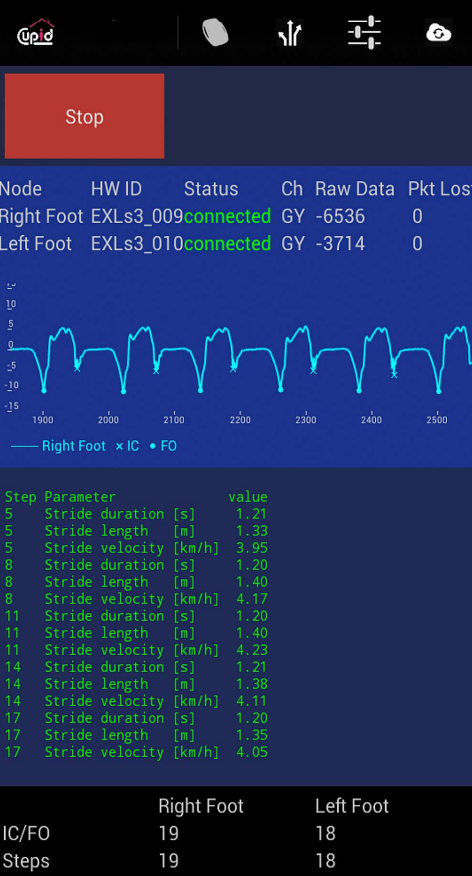
\includegraphics[width=0.5\textwidth]{img/Androidapp1.png}
        \caption{Captura de la apicación Android diseñada en \cite{7173053}}
        \label{fig:androidappmarcha}
    \end{figure}
    \item 'Unconstrained detection of freezing of Gait in Parkinson's disease patients using smartphone' \cite{7319209} propone una aplicación para dispositivos Android que permite recopilar los datos obtenidos con los sensores de acelerómetro y giroscopio presentes en el teléfono inteligente  Google Nexus 5  durante la marcha del paciente. Estos datos se procesan con el objetivo de clasificarlos entre episodios de congelación de la marcha y marcha normal. Esta aplicación tiene el propósito de detectar estos episodios, sin estar destinada al uso futuro de la misma por parte de un cliente.
    \item 'Feasibility and effects of home-based smartphone-delivered automated feedback training for gait in people with Parkinson's disease: A pilot randomized controlled trial' \cite{GINIS201628} presenta la aplicación CuPiD (Cueing and Prompting in Parkinson's Disease), diseñada para ayudar a los pacientes con Párkinson a controlar los episodios de congelación de la marcha y mejorar la calidad global de su marcha. Utiliza datos recogidos con sensores de movimiento sobre la marcha del paciente para proporcionar un feedback en tiempo real sobre la marcha del usuario y ofrecer instrucciones auditivas o visuales para mejorarla. Esta app demostró ser más eficaz en la mejora del equilibrio en pacientes con Párkinson que el entrenamiento de la marcha convencional.
\end{itemize}
\subsubsection{Análisis de la marcha en pacientes con enfermedades neurodegenerativas mediante dispositivos electrónicos portátiles}
El artículo 'Assessing Gait in Parkinson’s Disease Using Wearable Motion Sensors: A Systematic Review', escrito en 2019 por L. Brognara et al\cite{diseases7010018} se destaca la utilidad de las unidades de medición inercial (IMU), frecuentemente presentando funciones de acelerómetro y giroscopio, en el análisis objetivo de los movimientos en pacientes con enfermedades neurodegenerativas. Se destaca esta opción por la utilidad que presentan características como el reducido tamaño y coste de los mismos, que los hacen adecuados para el uso en contextos clínicos y fuera de ellos. En este texto se hace una revisión de artículos que posicionan los IMU en diferentes partes del cuerpo, siendo ambos tobillos la segunda localización más utilizada. \\

Este posicionamiento de sensores, así como la localización en la zona lumbar se utilizan en el artículo 'Wearables for gait and balance assessment in the neurological ward - study design and first results of a prospective cross-sectional feasibility study with 384 inpatients' \cite{Bernhard2018}, en el que se analiza el equilibrio y la marcha de pacientes neurológicos hospitalizados, la mayoría presentando patologías como Párkinson, ictus o leucemia. Se concluye la gran utilidad y fiabilidad de los dispositivos portables con acelerómetros 3D en la evaluación de estos parámetros en pacientes neurológicos.\\

\subsubsection{Líneas transversales en el suelo como ayuda visual al inicio de la marcha en pacientes con Párkinson}
El artículo 'Effects of visual and auditory cues on gait initiation in people with Parkinson's disease' \cite{doi:10.1191/0269215506cr925oa} describe la efectividad del uso de líneas transversales en la iniciación de la marcha de pacientes con Párkinson, destacando la mejora en la magnitud del inicio de la marcha: los pacientes que utilizan esta ayuda en el inicio de la marcha toman un primer paso con mayor fuerza, recorriendo una mayor longitud. Esto se mantiene a lo largo de la marcha, resultando en una velocidad promedio mayor.\\

Por otro lado, el artículo presentado por Chan et al.\cite{10.3389/fbioe.2024.1334403} investiga el efecto de la proyección de líneas láser como estímulo visual en pacientes con Párkinson. Se propone un dispositivo integrado en ambos zapatos del paciente, que utiliza la presión ejercida por el pie en la suela y la inercia para detectar el movimiento de cada pie, activando la proyección de línea láser en el pie contrario. De esta forma se proporciona en todo momento una ayuda visual al paciente durante la marcha. En pacientes con síntomas motores más agudos la ayuda de este dispositivo redujo la cantidad de episodios de congelación de la marcha.\\

El artículo presentado por Velik et al. \cite{6347005} describe que el uso de proyecciones de líneas láser paralelas en el suelo además de reducir significativamente la cantidad de episodios de congelación de la marcha, reduce su duración en un 51 por ciento con la proyección de líneas láser de forma continuada y un 69 por ciento con la proyección de líneas láser 'por demanda'.

\subsection{Proyectos relacionados}
\begin{itemize}
\item El artículo 'Gait monitoring system for patients with Parkinson’s disease' \cite{GONCALVES2021115653} presenta un sistema de monitorización de la marcha en pacientes con Párkinson, constituido por una unidad de medición inercial (IMU), con un sensor MPU-6050, el cual se utiliza para adquirir datos inerciales.\\

Este sensor se encuentra situado en un cinturón, que incluye también una unidad de almacenamiento de datos, una unidad de procesamiento con un algoritmo de detección de eventos de la marcha, el cual utiliza un microcontrolador Atmega 2560 y un módulo bluetooth. Este módulo se utiliza para comunicarse con una aplicación Android, que permite graficar los datos e iniciar/finalizar de forma inalámbrica el funcionamiento del dispositivo.
\item El artículo presentado por Takač et al. (2022)\cite{info:doi/10.2196/mhealth.2539} describe el uso de un sistema para la monitorización doméstica de la posición y orientación del paciente con Párkinson que sufre congelación de la marcha, proporcionando una base sólida para la detección de estos episodios. Para ello utiliza 2 tipos de sensores: por un lado sensores inerciales ubicados en un smartphone, que se sitúan junto al cuerpo del paciente (generalmente en la cintura) y por otro lado cámaras RGB-D para obtener un contexto 3D del ambiente en que se encuentra el paciente, los cuales habitualmente se colocan en las esquinas de la habitación donde se quiere realizar la monitorización. \\
Se empleó software especializado para la recopilación de datos, clasificación de la posición del paciente y seguimiento de objetos. Los resultados mostraron una gran precisión en la detección de la posición y orientación del paciente, mostrando por tanto una alta fiabilidad para la monitorización de Párkinson tanto en entornos clínicos como domésticos.

\end{itemize}
\capitulo{4}{Metodología}

\section{Descripción de los datos.}
Conforme a los previos TFGs relacionados con el presente proyecto \cite{Gonzalez2023} \cite{Martos2024} se  mantuvo la utilización de los datos obtenidos durante la realización de actividades a partir del sensor MPU-6050 para enviar, mediante el script Arduino, datos relevantes como el número de bloqueos, la velocidad media, el número de pasos o la duración de la actividad hacia el servidor web Node.js, por medio del script bridge.py (que funciona como enlace entre el servidor y script Arduino previamente mencionados). \\

Adicionalmente, dentro de la función de guardado de actividades en la base de datos que presenta Node.js, se generaron las variables de fecha y hora, que registran la fecha y hora actuales durante la finalización y guardado de la actividad. Debido a esto, se modificó la tabla 'actividades' de la base de datos 'webparkinson', añadiendo las columnas 'fecha' (de tipo 'DATE') y hora (de tipo 'TIME').\\

El registro de los datos obtenidos en los diarios de tomas de medicación y fluctuaciones de los pacientes que el paciente rellena en la página web requirieron la creación de 2 tablas adicionales en la base de datos: diario y diario2.
\begin{itemize}
    \item La tabla 'diario' registra los datos relativos a las fluctuaciones del paciente. Consta de 6 columnas, fecha, hora y 4 columnas correspondientes a los diferentes estados del paciente a lo largo del día: durmiendo, off, on y on con discinesia. Cada hora del día para la cual se registra un estado en el diario de fluctuaciones se corresponderá con 1 fila en esta tabla. Al tratarse de un cuestionario en que el estado de cada hora se rellena tan sólo con un tick, el valor del estado seleccionado será 1 y el valor del resto de estados 0.
    \item La tabla 'diario2' registra los datos relativos a la toma de medicaciones diaria por parte del paciente. Consta de 8 columnas: id de la tabla (clave primaria), fecha, medicación y 5 columnas de tipo 'time' para el registro de las horas de toma de dicha medicación. Cada medicación registrada en el diario se corresponderá con 1 fila de esta tabla. En caso de que 1 medicación tenga un número menor que 5 tomas diarias, las columnas correspondientes a las tomas restantes se rellenarán con el valor 'NULL' (nulo).
\end{itemize}
Los datos registrados en las 3 actividades mencionadas, son utilizados en los archivos grafdiarios.py con el objetivo de visualizar las fluctuaciones motoras y tomas de medicaciones de una fecha concreta y graficasmed.py para comparar los bloqueos/min producidos en actividades realizadas durante intervalos on, on con discinesia y off.\\

Adicionalmente, se creó una última tabla para el almacenamiento de las pruebas de personalización del tiempo de bloqueo. Esta tabla tiene una estructura idéntica a la tabla de actividad, omitiendo las columnas de fecha y hora. Sin embargo, necesita almacenarse de manera separada para el posterior cálculo del tiempo de reposo óptimo para identificar un congelamiento de la marcha acorde con la prueba y el envío de dicho número de segundos al script de Arduino.

 
\section{Técnicas y herramientas.}
\subsection{Técnica de desarrollo software}
El objetivo principal del desarrollo software durante este proyecto ha sido la adición de diversas funcionalidades a la aplicación web y al script Arduino para una mayor utilidad de la app. A pesar de haber realizado una planificación inicial dejando unos claros objetivos principales de desarrollo, el uso en este proyecto de diversos lenguajes de programación, bibliotecas y plataformas daba pie a un amplio rango de opciones de desarrollo de estos objetivos. \\
Teniendo en cuenta la clasificación de proyectos descrita en \ref{fig:clasificacionproyectos}, este proyecto se situaría en el grupo 2: objetivo claro y solución poco conocida. Este grupo requiere métodos que permitan la evolución de ideas a lo largo del desarrollo del proyecto, a partir de ciclos de retroalimentación.\cite{Pradel2013}\\
\begin{figure}[h]
    \centering
    \includegraphics[width=1\textwidth]{img/Clasificaciónproyectos.png}
    \caption{Esquema de clasificación de proyectos de desarrollo software \cite{Pradel2013}}
    \label{fig:clasificacionproyectos}
\end{figure}
Teniendo en cuenta que las funcionalidades marcadas como objetivo podían ser divididas en grupos, cuyo correcto funcionamiento es independiente del resto de grupos, era factible la posibilidad de realizar iteraciones en el ciclo de desarrollo.\\
Debido a ello, y con el objetivo de mantener una mayor flexibilidad a la hora de escoger el enfoque adecuado para cada objetivo a lo largo del proyecto, así como de cubrir la necesidad de realizar exhaustivas pruebas para cada funcionalidad desarrollada, se decidió optar por una metodología de desarrollo ágil: el ciclo de vida iterativo e incremental.
\subsection{Ciclo de vida iterativo e incremental}
Los métodos iterativos distribuyen el desarollo software en una serie de iteraciones, que constituyen en sí mismos pequeños proyectos, ampliando las funcionalidades de la iteración anterior. Recorrer todas las fases del desarrollo del producto en cada iteración (requisitos, análisis, implementación y pruebas) presenta 2 ventajas principales\cite{Pradel2013}:
\begin{itemize}
    \item Retroalimentación constante: La obtención de información sobre el funcionamiento del código implementado en cada iteración permite una detección precoz de posibles errores o potenciales mejoras en el código implementado, permitiendo en posteriores iteraciones una mejora informada de la utilidad de las funciones previas adicional al incremento de funcionalidades.
    \item Producto operativo en todo momento: Al contrario que otras metodologías de desarrollo software, como el desarrollo en cascada, en que el producto sólo es funcional y operativo al finalizar el proyecto, este método nos permite obtener diferentes versiones funcionales del producto a lo largo del desarrollo.
\end{itemize}
Un ciclo de vida iterativo incluye entre las fases de planificación inicial y despliegue final del producto un ciclo de desarrollo que se repite constantemente, tal y como se muestra en la figura \ref{fig:iterativoincremental}.
\begin{figure}[h]
    \centering
    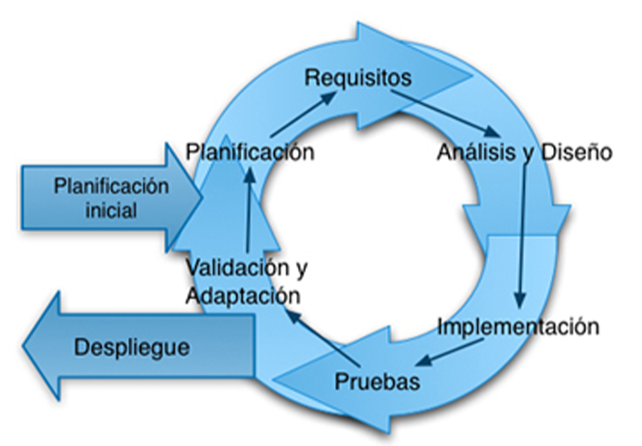
\includegraphics[width=0.7\textwidth]{img/Iterativoincremental.png}
    \caption{Ciclo de vida del desarrollo software iterativo \cite{Pradel2013} }
    \label{fig:iterativoincremental}
\end{figure}
Cada iteración durará entre 1 y 6 semanas, siendo ideal mantener una duración uniforme entre las distintas iteraciones. Al finalizar cada iteración, se tendrán en cuenta los resultados obtenidos para adaptar la planificación, requisitos y demás fases de las iteraciones posteriores.\\
A lo largo de este proyecto se realizaron 5 iteraciones de desarrollo software (partiendo del desarrollo software en el TFG \cite{Martos2024}), resultando la duración de las mismas algo dispar debido a complicaciones técnicas que se produjeron en algunas de ellas:
\begin{itemize}
    \item Primera iteración (semanas 1-2): generación de gráficas a partir de las actividades almacenadas en la base de datos. Generación y descarga automática de informe médico incluyendo dicha información de actividades y de forma opcional las gráficas. Para realizar pruebas durante esta iteración se utilizó el prototipo hardware construido en el TFG \cite{Martos2024}.
    \item Segunda iteración (Semanas 3-4): Personalización del tiempo de reposo que el script Arduino detecta como congelación de la marcha mediante la realización de una sencilla prueba. Para probar los resultados de esta iteración también se utilizó el prototipo hardware construido en el TFG \cite{Martos2024}.
    \item Tercera iteración (Semenas 5-10): Implementación de un diario de fluctuaciones motoras. Mejora de las funcionalidades anteriores. Se realizaron las pruebas de funcionamiento de dichas mejoras utilizando Protoboards de Arduino como montaje provisional del nuevo hardware.
    \item Cuarta iteración (Semanas 11-13): Almacenamiento de datos del diario de fluctuaciones en la base de datos, registro de la hora y fecha de las actividades realizadas. Las pruebas de esta iteración pudieron realizarse en un modelo definitivo del nuevo hardware.
    \item Quinta iteración (Semanas 14-15): Gestión de los datos de actividades registradas y diarios para la realización de gráficas relevantes sobre los mismos. Pruebas finales de funcionamiento.
\end{itemize}
\subsection{Herramientas software}
\begin{itemize}
    \item XAMPP: Herramienta que permite la instalación de un servidor web en el dispositivo. En concreto se han utilizado los componentes del servidor web Apache y MySQL. Ha resultado útil para continuar el desarrollo de la aplicación web de forma local.
    \begin{itemize}
    \item MySQL: Este componente de XAMPP permite la gestión de bases de datos de forma local. Se ha utilizado para generar tablas para el almacenamiento de datos del diario de tomas y de fluctuaciones motoras.
    \end{itemize}
    \item Visual Studio Code: Aplicación para el desarrollo de código que permite la utilización de diferentes lenguajes de programación dentro de la misma. Se ha utilizado para generar archivos .php, en los cuales se incluyó código HTML y Javascript, así como para la edición de archivos .js que manejan la comunicación bidireccional entre la aplicación web y el código de Arduino.
    \item IDE Arduino: Entorno de desarrollo software para la escritura, compilación y carga de código en placas de Arduino. Se utilizó para modificar el script Arduino, incluyendo la personalización de bloqueos, el manejo del módulo láser...
    \item Autodesk Sketchbook: Software utilizado para el desarrollo de planos del hardware a desarrollar.
    \item Microsoft Visio: Software de diagramación utilizado para ilustrar las conexiones entre los componentes hardware y la placa Arduino Uno.
    \item Microsoft Excel: Software de hojas de cálculo que ha sido utilizado para la realización de los diagramas de Gantt que ilustran la planificaicón del proyecto.
    \item Versión 2 de ChatGPT: IA de conversación creada por OpenAI que ha sido utilizada en ocasiones como apoyo durante el desarrollo de software.
    \item Lucidchart: Software de creación de diagramas online utilizado para la creación de diagramas incluidos en los Anexos.
    \item Balsamiq Wireframes: Software de creación de prototipos de interfaces y wireframes, que ha sido utilizada para la creación de los wireframes de la página web incluidos en los Anexos.
    \item Visual paradigm: Software de creación online de diagramas UML, utilizado para la creación del diagrama de despliegue incluido en los anexos.
    \item Tinkercad: software online que permite crear diseños 3D así como crear y simular el funcionamiento de circuitos electrónicos. Se utilizó para ilustrar la conexión de algunos componentes hardware a la placa Arduino en los anexos.
\end{itemize}
\subsubsection{Lenguajes de programación}
\begin{itemize}
    \item PHP: Este lenguaje de programación permite el desarrollo backend en aplicaciones web. Se utilizó mayoritariamente como enlace entre los formularios mostrados en pantalla y la base de datos, recogiendo al enviarse el formulario los datos insertados e insertándolos en filas de la tabla correspondiente en la base de datos. Adicionalmente se utilizó de forma complementaria en los documentos destinados al desarrollo frontend para realizar funciones complejas no realizables mediante HTML.
    \item Javascript: Este lenguaje permite la creación de contenido dinámico e interactivo en aplicaciones web. Se utilizó principalmente para otorgar dinamismo a formularios web en el frontend.
    \item HTML: Este lenguaje permite la creación de contenido estático en aplicaciones web. Se utilizó principalmente en el desarrollo de formularios para el registro diario de fluctuaciones y tomas, complementándolo con el uso de CSS para manejar el estilo del contenido.
    \item Python: Este lenguaje de programación se utilizó para generación de pdfs y gráficas a partir de las actividades registradas.
    \item Arduino C/C++: El lenguaje de programación utilizado en IDE Arduino, constituye una variante simplificada de los lenguajes de programación C/C++.
\end{itemize}
\subsubsection{Bibliotecas utilizadas en los distintos lenguajes de programación}
\begin{enumerate}
    \item \textbf {Bibliotecas de python utilizadas para la generación de PDFs}
        \begin{itemize}
            \item 'Reportlab': Biblioteca para la generación de documentos PDF. En los archivos 'pdf.py' y 'pdf2.py' se utilizaron los siguientes submódulos o clases de esta bibioteca:
            \begin{itemize}
                \item 'reportlab.lib.pagesizes.letter'
                \item 'reportlab.platypus.SimpleDocTemplate'
                \item 'reportlab.platypus.Paragraph'
                \item 'reportlab.platypus.Spacer'
                \item 'reportlab.platypus.Table'
                \item 'reportlab.lib.styles.getSampleStyleSheet'
                \item 'reportlab.lib.colors'
                \item 'reportlab.platypus.Image'
            \end{itemize}
            \item 'Urllib': Biblioteca que permite trabajar con URLs. En concreto, se usó la función 'urllib.request.urlretrieve', que permite descargar archivos desde una URL y guardarlos correctamente.
            \item 'os': Biblioteca para interactuar con el sistema operativo.
            \item 'json': Biblioteca que permite trabajar con datos JSON.
            \item 'mysql.connector': Biblioteca para la conexión e interacción con bases de datos MySQL.
        \end{itemize}
    \item \textbf {Bibliotecas/funciones de python utilizadas para la generación de gráficas}
            \begin{itemize}
                \item 'os': Biblioteca para interactuar con el sistema operativo.
                \item 'sys': Funciones y variables que interactúan con el intérprete de python.
                \item 'json': Biblioteca que permite trabajar con datos JSON.
                \item 'matplotlib.pyplot': herramienta para la creación de gráficas.
                \item 'Ipython.display': funciones que permiten mostrar contenidos multimedia en notebooks de python.
                \item 'mysql': Paquete que permite interactuar con bases de datos MySQL. Dentro del mismo, se utilizan las funciones 'mysql.connector' para conectar y ejecutar consultas con bases de datos MySQL.
                \item 'pandas': Biblioteca para la manipulación y análisis de datos de tablas.
                \item 'sqlalchemy': Biblioteca que permite conectarse con bases de datos relacionales con la función 'create engine', que crea un motor o representación abstracta de la base de datos a la cual se conecta con sqlalchemy.
            \end{itemize}
    \item \textbf {Bibliotecas/funciones de otros lenguajes de programación }
Como bibliotecas y funciones de los lenguajes de programación PHP y Arduino se utilizaron principalmente los recursos descritos en el TFG \cite{Martos2024}. Se utilizó también la biblioteca de Arduino 'RTClib.h' durante los intentos de inclusión del módulo RTC en el hardware. Sin embargo, como se describe en el apartado 'Conclusiones', esta biblioteca no se utiliza en el prototipo presentado debido a la decisión de no incluir dicho módulo.
\end{enumerate}



\subsection{Herramientas hardware}
Se reconstruyó el hardware presentado en el TFG \cite{Martos2024}, incluyendo también un módulo láser y rediseñando el prototipo para insertarlo en un cinturón y tobillera, como se muestra en la figura \ref{fig:esquemahardware}. En esta imagen podemos observar una primera banda, en la que se representan los componentes adheridos a la zona exterior del cinturón, una segunda banda con los componentes adjeridos a la zona interior del cinturón y el sensor MPU-6050, insertado en la tobillera y comunicado con el cinturón mediante un cable multihilo. 
El circuito de conexión de los componentes hardware a la placa Arduino se realizó mediante el Arduino proto shield, siguiendo el esquema mostrado en la figura \ref{fig:esquemacircuito}. Adicionalmente a las conexiones representadas en esta figura, se alimentó la placa Arduino mediante una batería. Esta alimentación se controlaba mediante el interruptor ON/OFF (la conexión de estos componentes puede observarse también en la figura \ref{fig:esquemahardware}).
\begin{figure}[h]
    \centering
    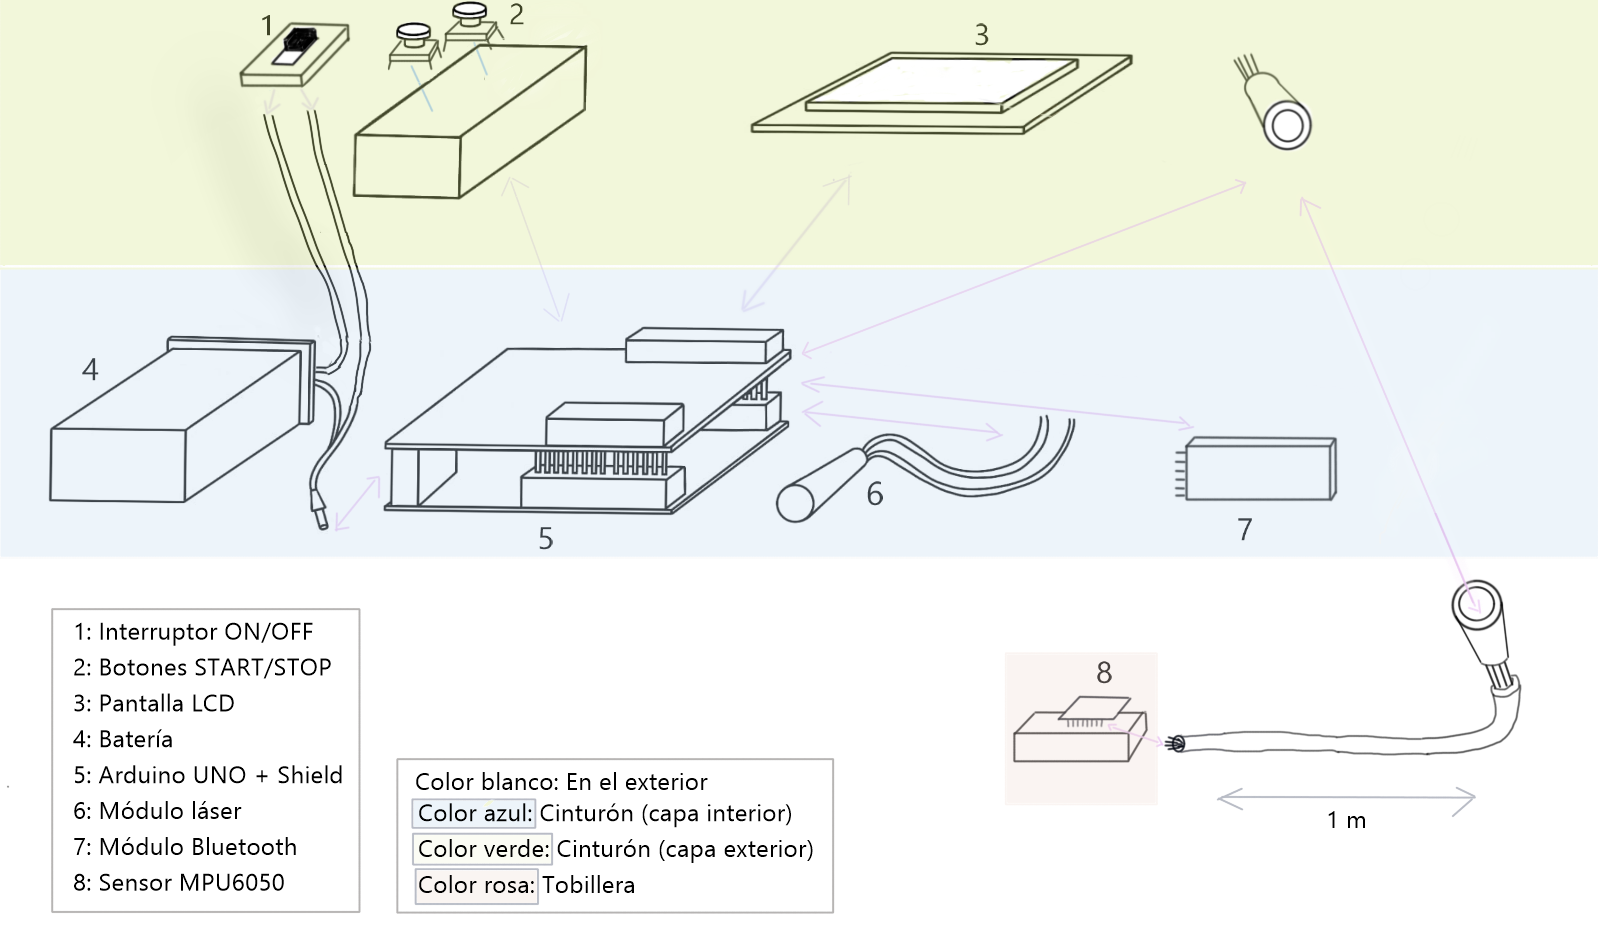
\includegraphics[width=1\textwidth]{img/esquemahardware.png}
    \caption{Esquema de la colocación de elementos hardware en el prototipo}
    \label{fig:esquemahardware}
\end{figure}
\begin{sidewaysfigure}[h]
    \centering
    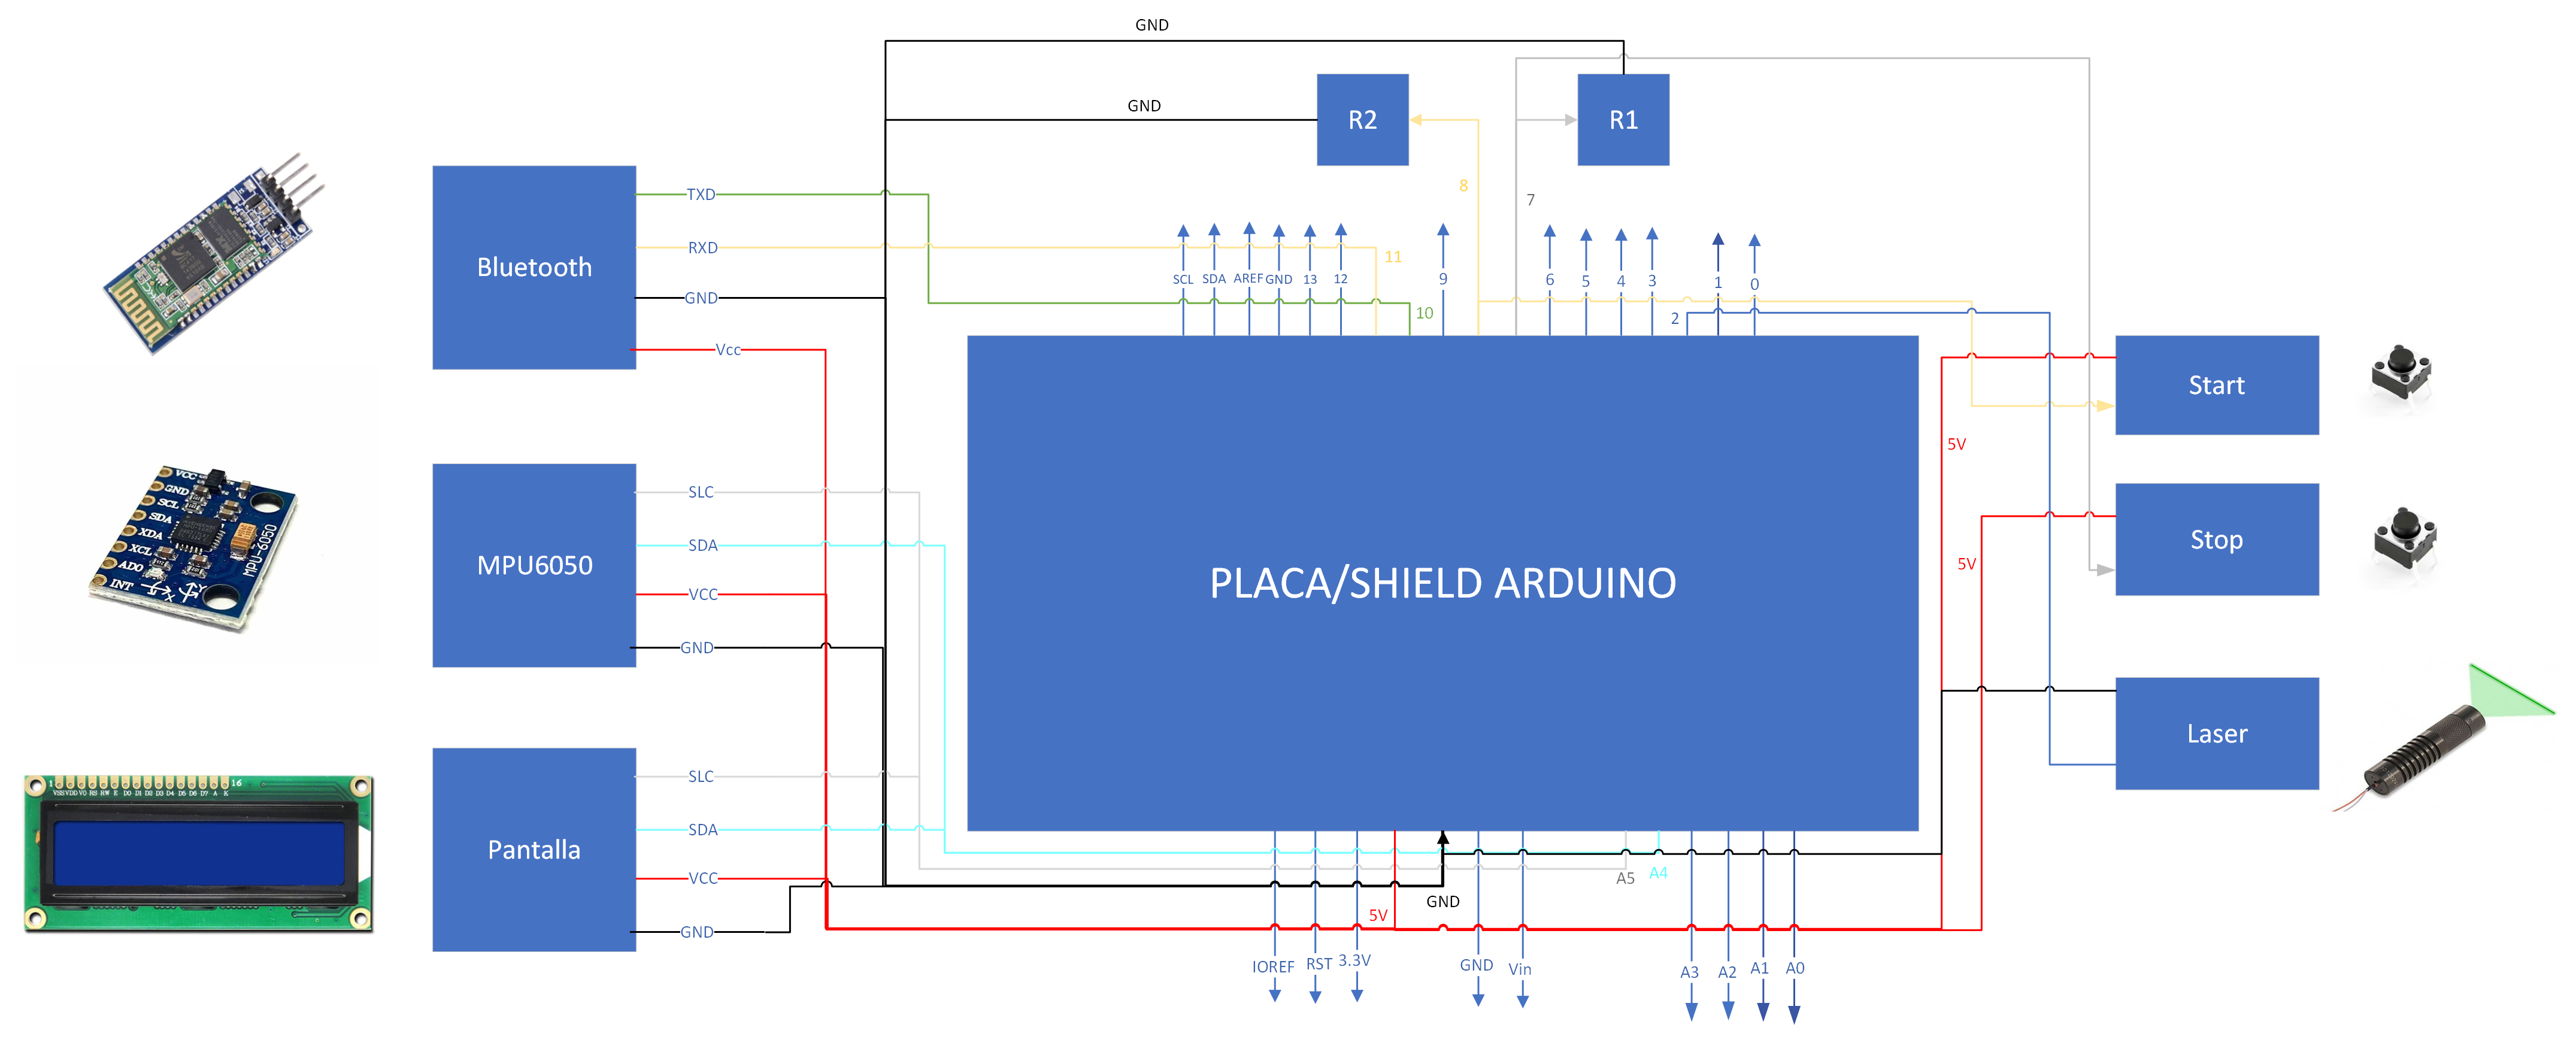
\includegraphics[width=1\textwidth]{img/circuito.png}
    \caption{Esquema del circuito formado por la placa Arduino UNO y los componentes conectados a la misma}
    \label{fig:esquemacircuito}
\end{sidewaysfigure}
Los componentes hardware utilizados para el diseño de este prototipo fueron:
\begin{itemize}
\item Microcontrolador Arduino UNO R3: Microcontrolador Arduino basado en ATmega328P, que consta de 14 pines digitales, 6 pines analógicos, conexión USB y toma de corriente.\ref{fig:unor3}
\begin{figure}
    \centering
    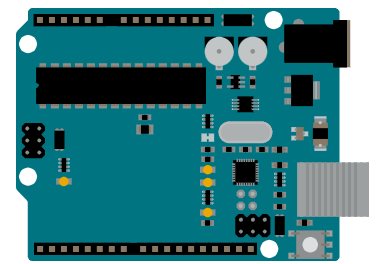
\includegraphics[width=0.5\textwidth]{img/unor3.png}
    \caption{Arduino UNO R3}
    \label{fig:unor3}
\end{figure}
\item Fuente de alimentación 9V
\item Interruptor ON/OFF
\item Pantalla LCD 16x2 con módulo LCD I2C \ref{fig:pantalla}: Esta pantalla de permite la visualización simultánea de 2x16 caracteres. El módulo LCD nos permite conectar con la pantalla empleando tan sólo 4 pines, haciendo más sencilla la integración en el circuito. \begin{figure}[h]
    \centering
    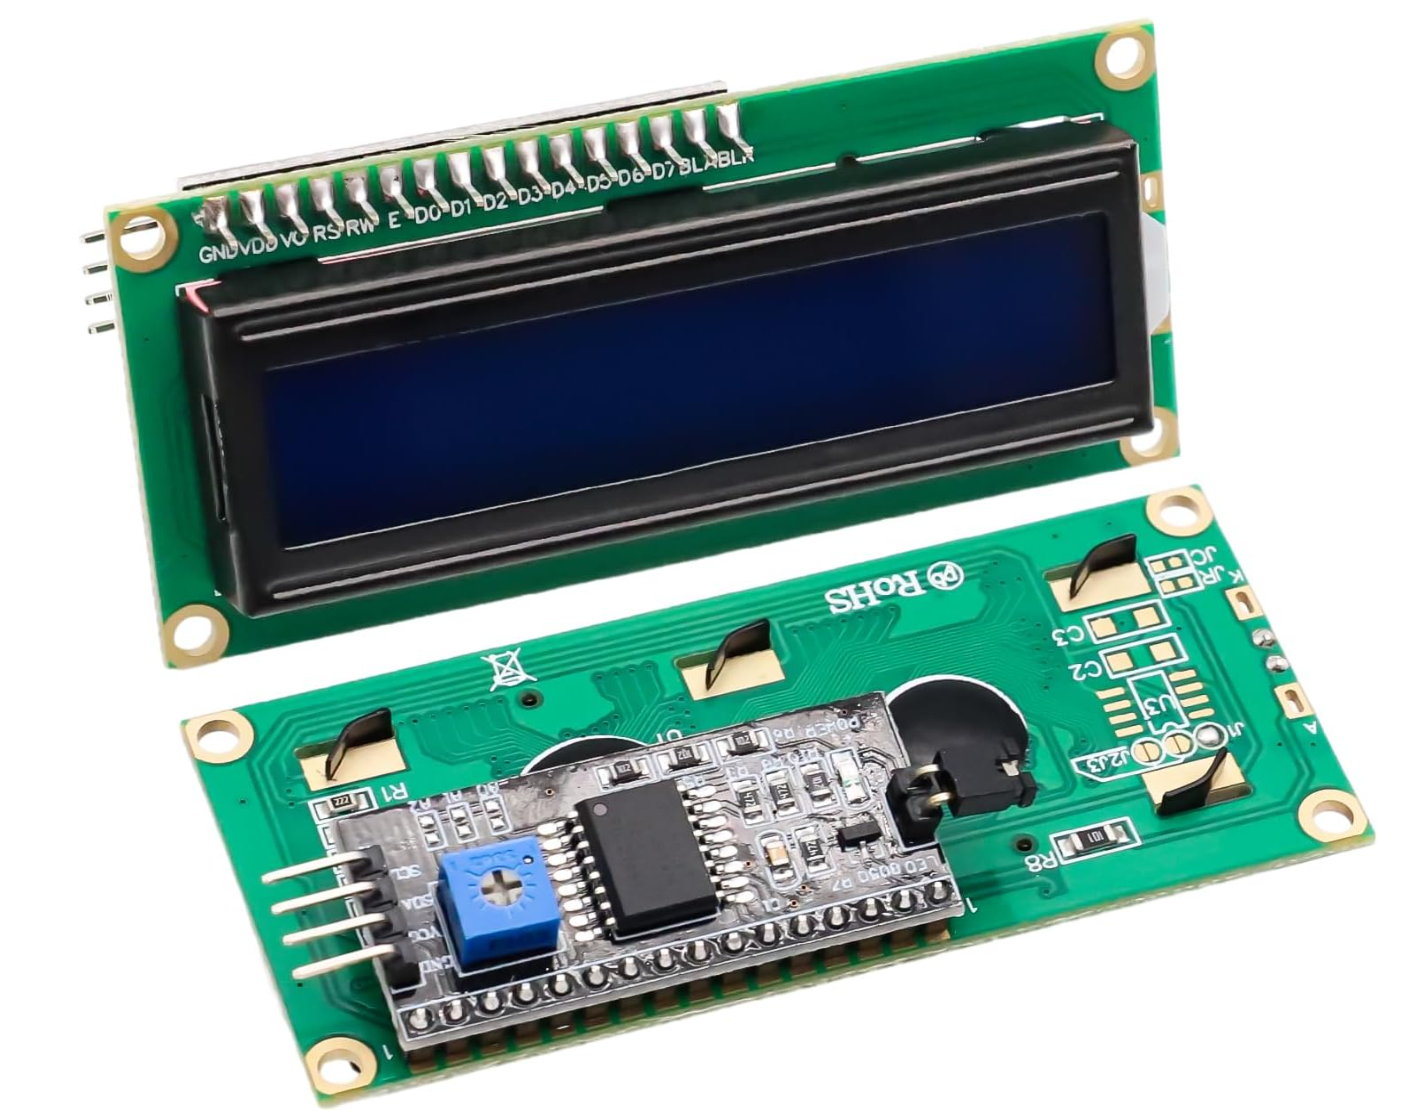
\includegraphics[width=0.8\textwidth]{img/pantalla.png}
    \caption{Pantalla LCD 16x2 con módulo LCD I2C \cite{ARCELI_LCD_Module}}
    \label{fig:pantalla}
\end{figure}
\item 2 pulsadores: Se utilizaron 2 pulsadores como botones de start/stop del dispositivo.
\item Módulo láser \ref{fig:laser}: Se incluyó un módulo láser que proyecta una línea recta en el suelo como respuesta a la detección de un congelamiento de la marcha.
\begin{figure}
    \centering
    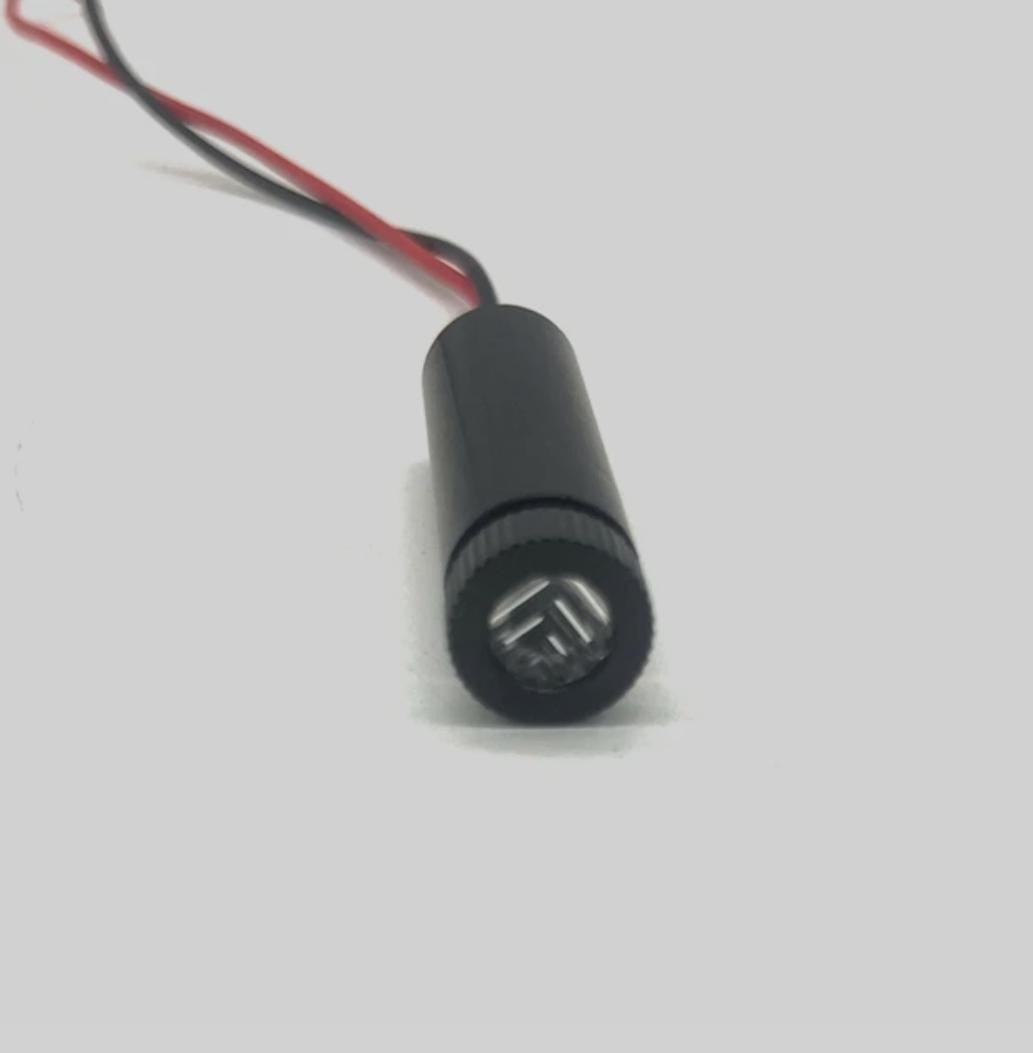
\includegraphics[width=0.5\textwidth]{img/laser.jpg}
    \caption{Módulo láser. \cite{LaserModule}}
    \label{fig:laser}
\end{figure}
\item Módulo bluetooth HC-05 \ref{fig:bluetooth}: Se utilizó este módulo de comunicación bluetooth serial para permitir la conexión inalámbrica entre el dispositivo y la aplicación web.
\begin{figure}
    \centering
    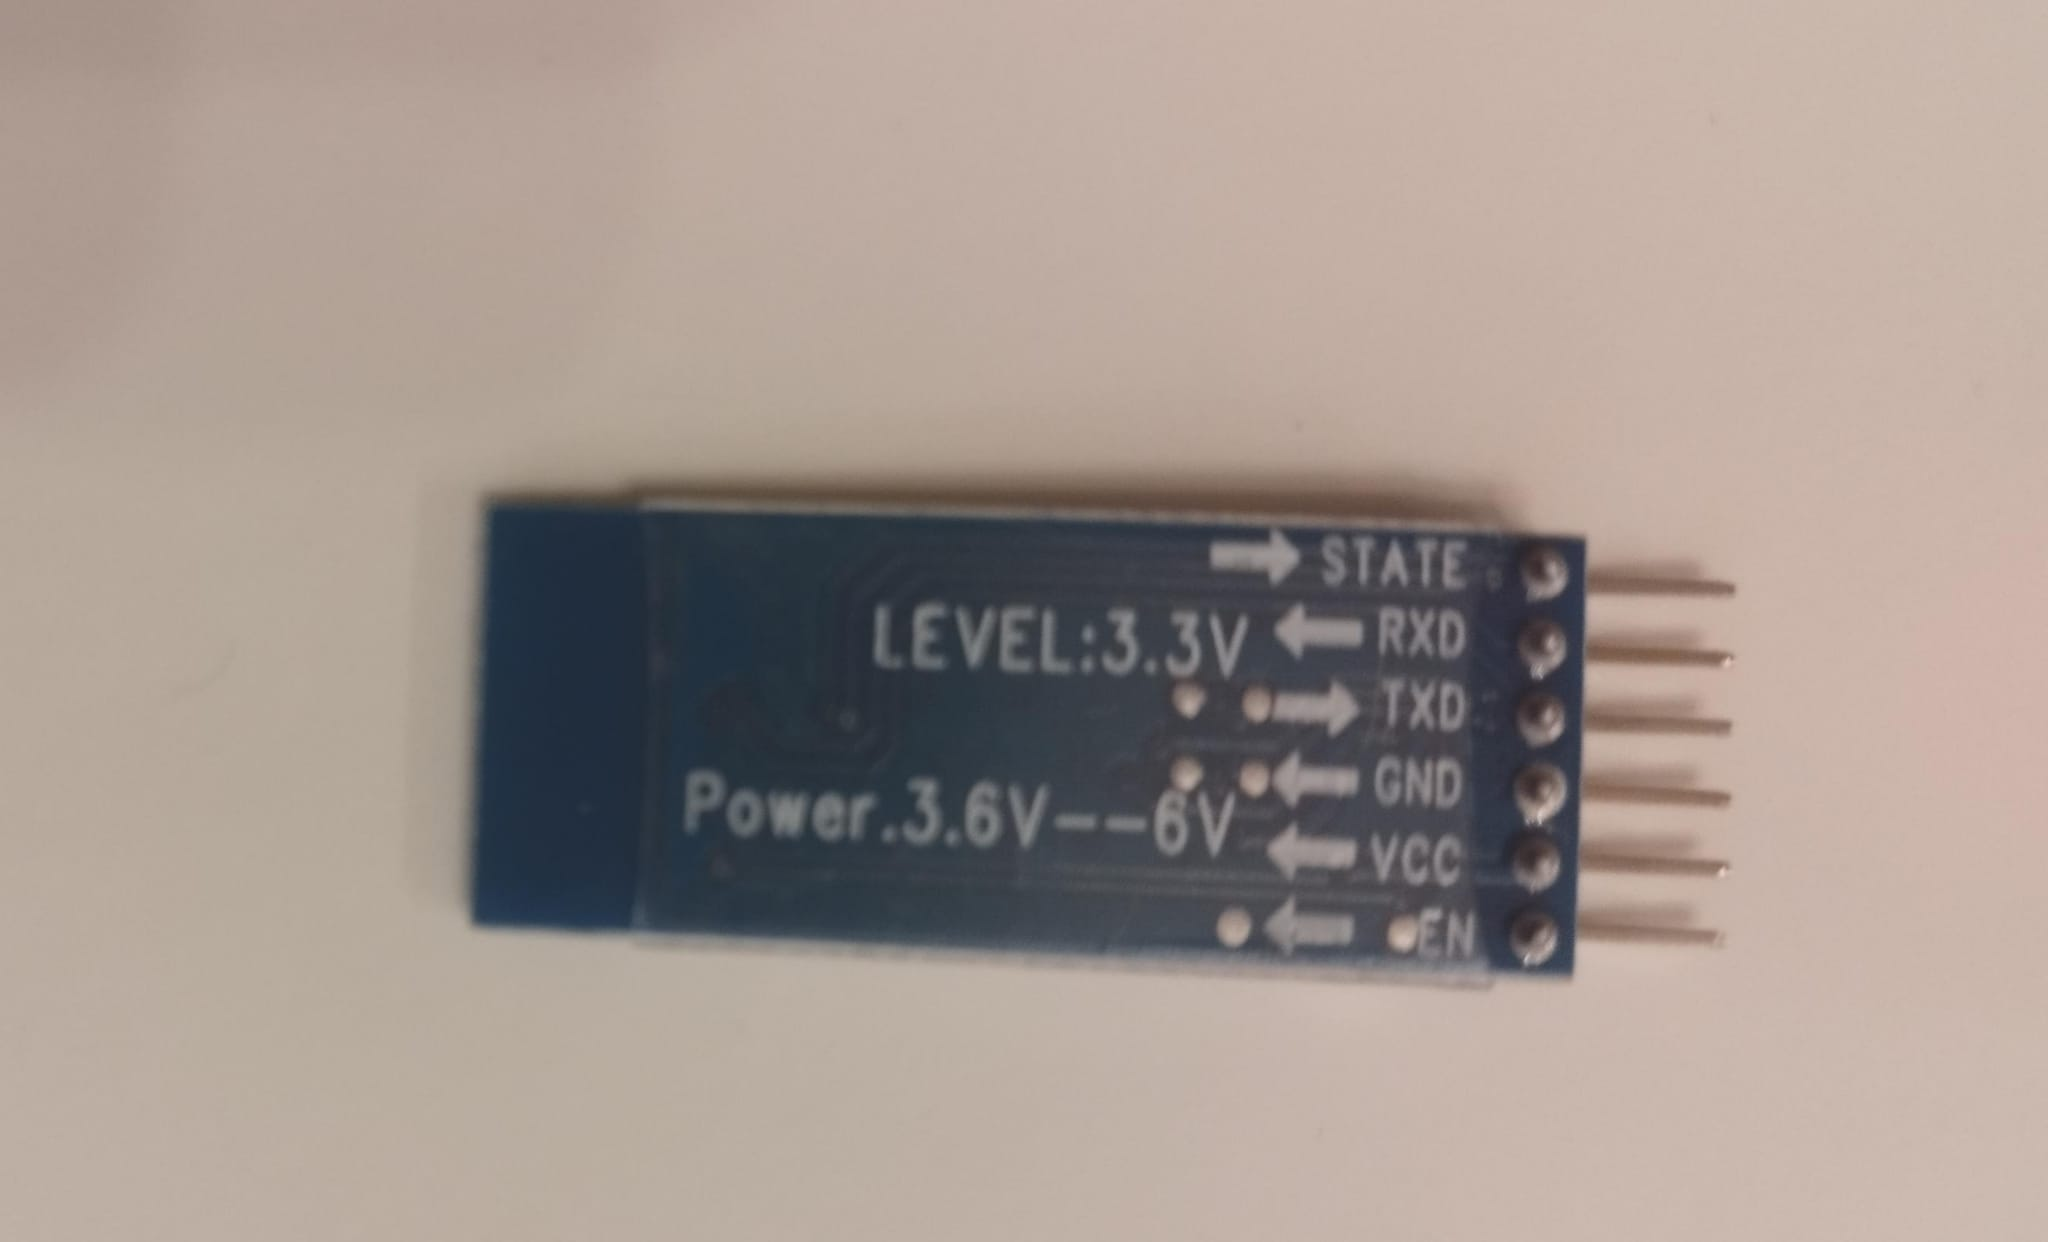
\includegraphics[width=0.5\textwidth]{img/bluetooth.jpg}
    \caption{Módulo bluetooth HC-05}
    \label{fig:bluetooth}
\end{figure}
\item Cable multihilo: como conexión entre el cinturón y la tobillera se utilizó un cable multihilo
\item Sensor MPU-6050 \ref{fig:mpu}: Se utilizó este sensor de movimiento y giroscopio de seis ejes para recoger los datos del acelerómetro y giroscopio relacionados con la marcha del paciente.

\begin{figure}
    \centering
    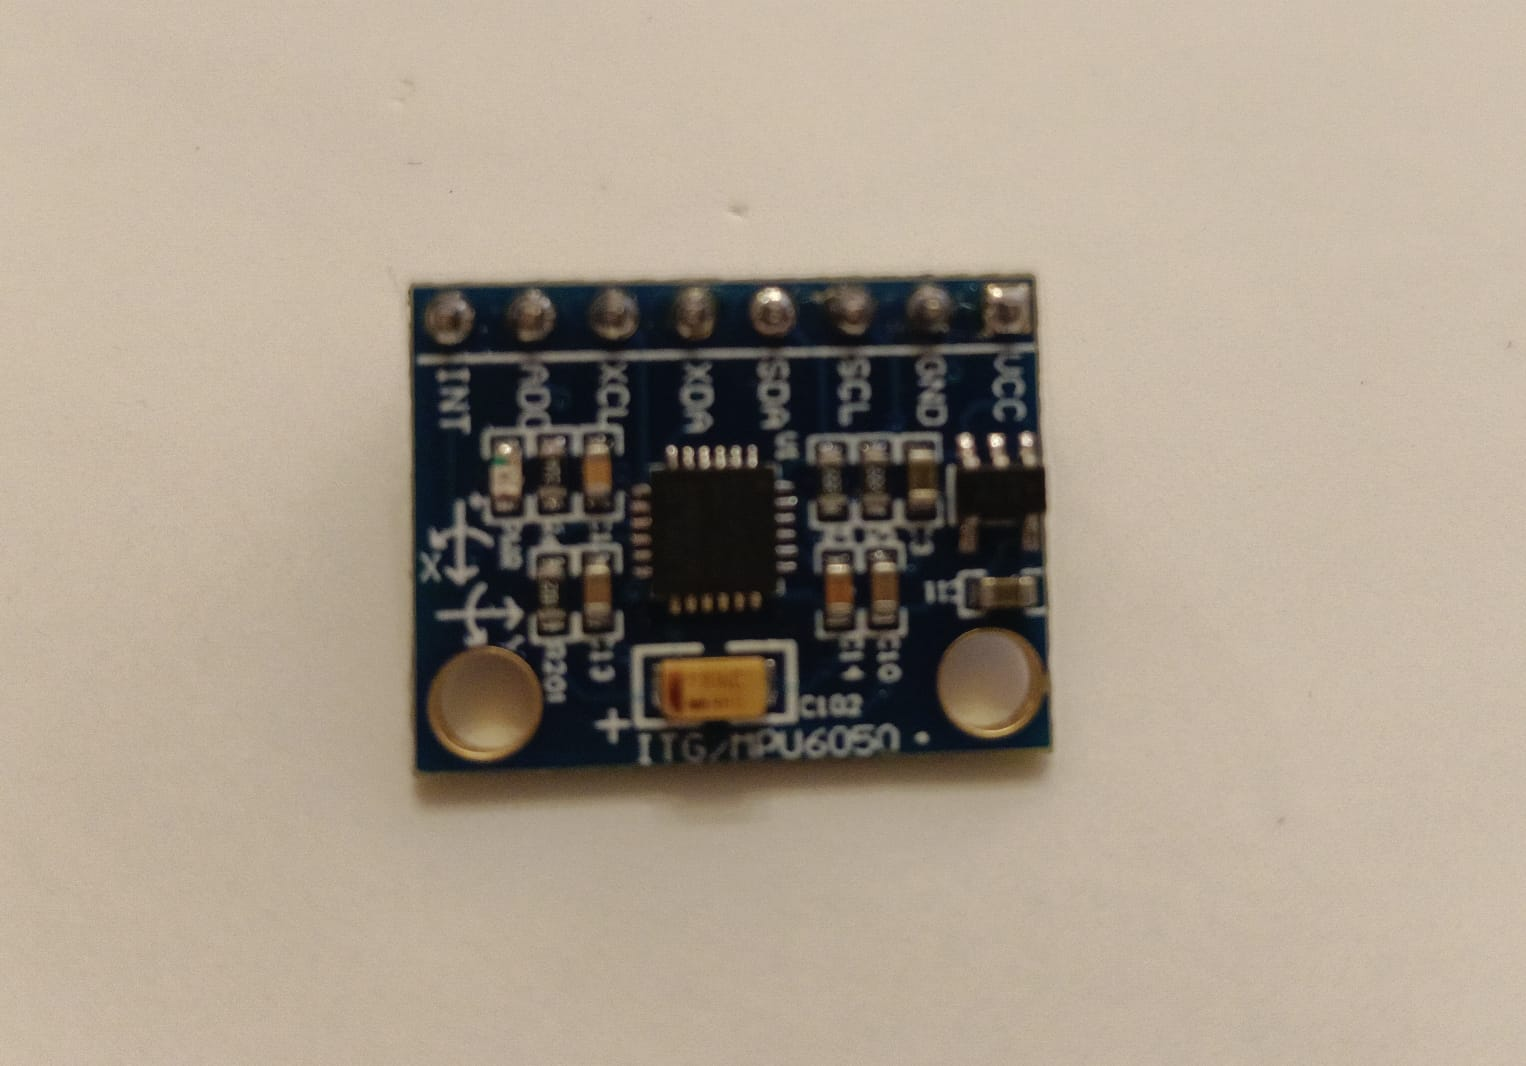
\includegraphics[width=0.5\textwidth]{img/mpu6050.jpg}
    \caption{Sensor MPU-6050. Fuente propia.}
    \label{fig:mpu}
\end{figure}
\end{itemize}
%Esta parte de la memoria tiene como objetivo presentar las técnicas metodológicas y las herramientas de desarrollo que se han utilizado para llevar a cabo el proyecto. Si se han estudiado diferentes alternativas de metodologías, herramientas, bibliotecas se puede hacer un resumen de los aspectos más destacados de cada alternativa, incluyendo comparativas entre las distintas opciones y una justificación de las elecciones realizadas. 
%No se pretende que este apartado se convierta en un capítulo de un libro dedicado a cada una de las alternativas, sino comentar los aspectos más destacados de cada opción, con un repaso somero a los fundamentos esenciales y referencias bibliográficas para que el lector pueda ampliar su conocimiento sobre el tema.

 


\capitulo{5}{Resultados}

\section{Resumen de resultados.}
El presente proyecto presenta un prototipo hardware/software funcional, el cual tiene un gran potencial para servir como ayuda tanto al paciente con párkinson como al profesional sanitario. Provee al paciente una ayuda visual en tiempo real para superar rápidamente y de mejor manera los congelamientos de la marcha, los cuales se detectan de forma personalizada para adecuarse a las características del usuario. También proporciona avances en el análisis de la evolución de la enfermedad, permitiendo descargar informes con los datos recogidos, visualizar gráficas sobre dichos datos y tener en cuenta la percepción del paciente sobre sus fluctuaciones motoras.

El trabajo realizado ha completado los objetivos hardware propuestos en cuanto a la creación de un nuevo prototipo incluyendo un módulo láser y diseñado dicho hardware de forma más cómoda que en previos prototipos, insertando los componentes en un cinturón y una tobillera, como se muestra en las imágenes \ref{fig:prototipo} \ref{fig:prototipoencendido}.

\begin{figure}[h]
    \centering
    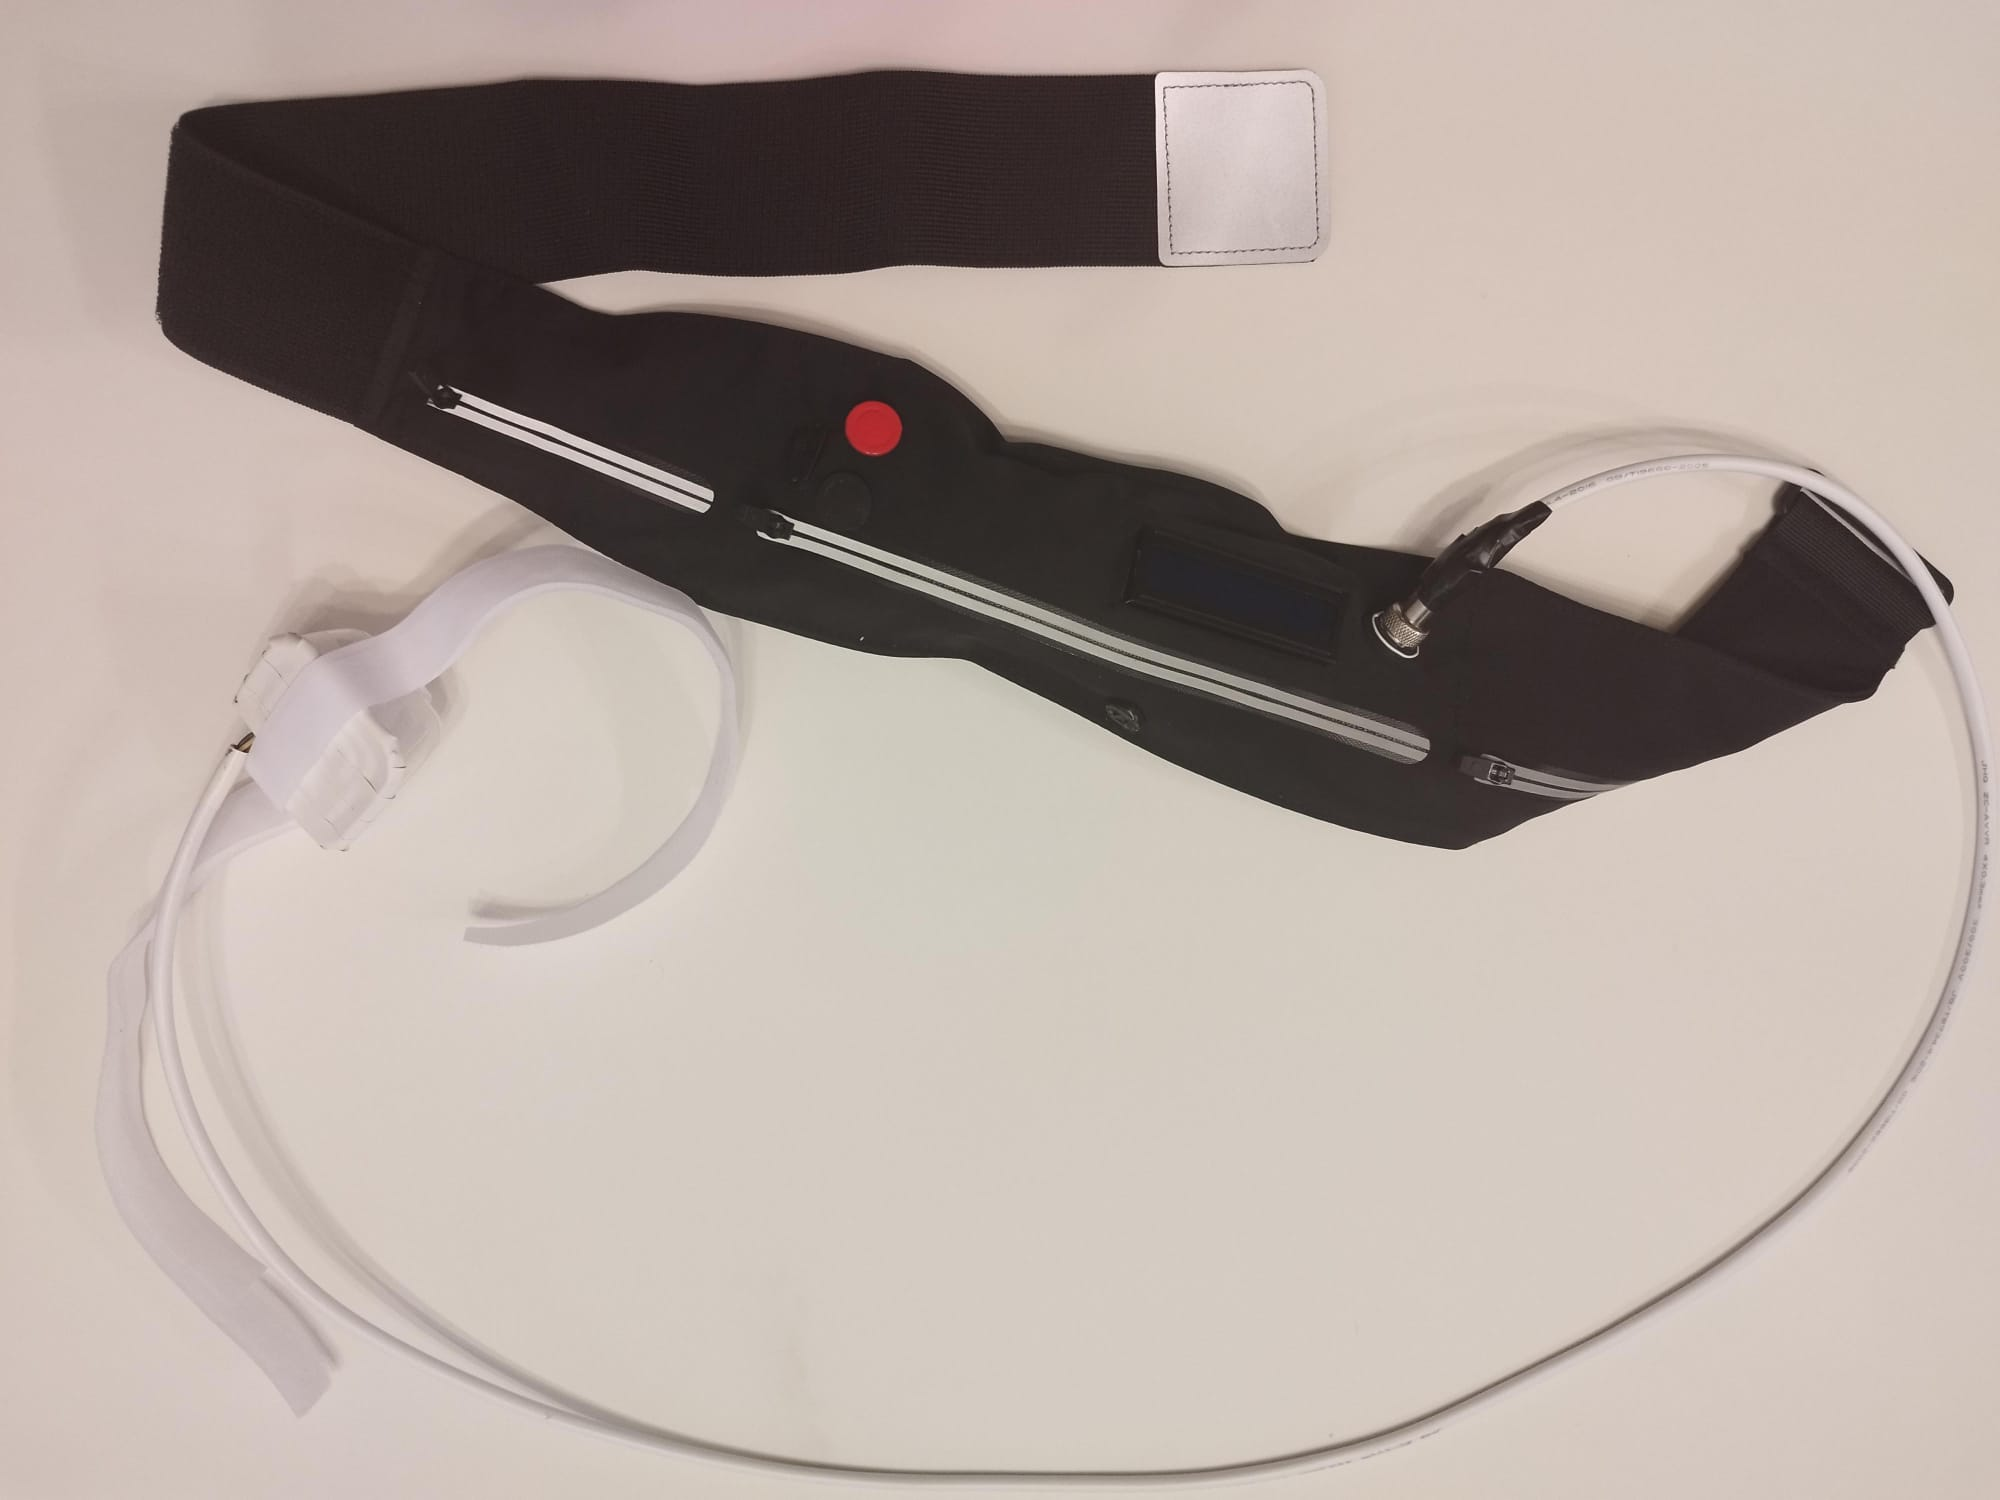
\includegraphics[width=1\textwidth]{img/prototipocompleto.jpg}
    \caption{Prototipo hardware completo. Fuente propia.}
    \label{fig:prototipo}
\end{figure}

\begin{figure}[h]
    \centering
    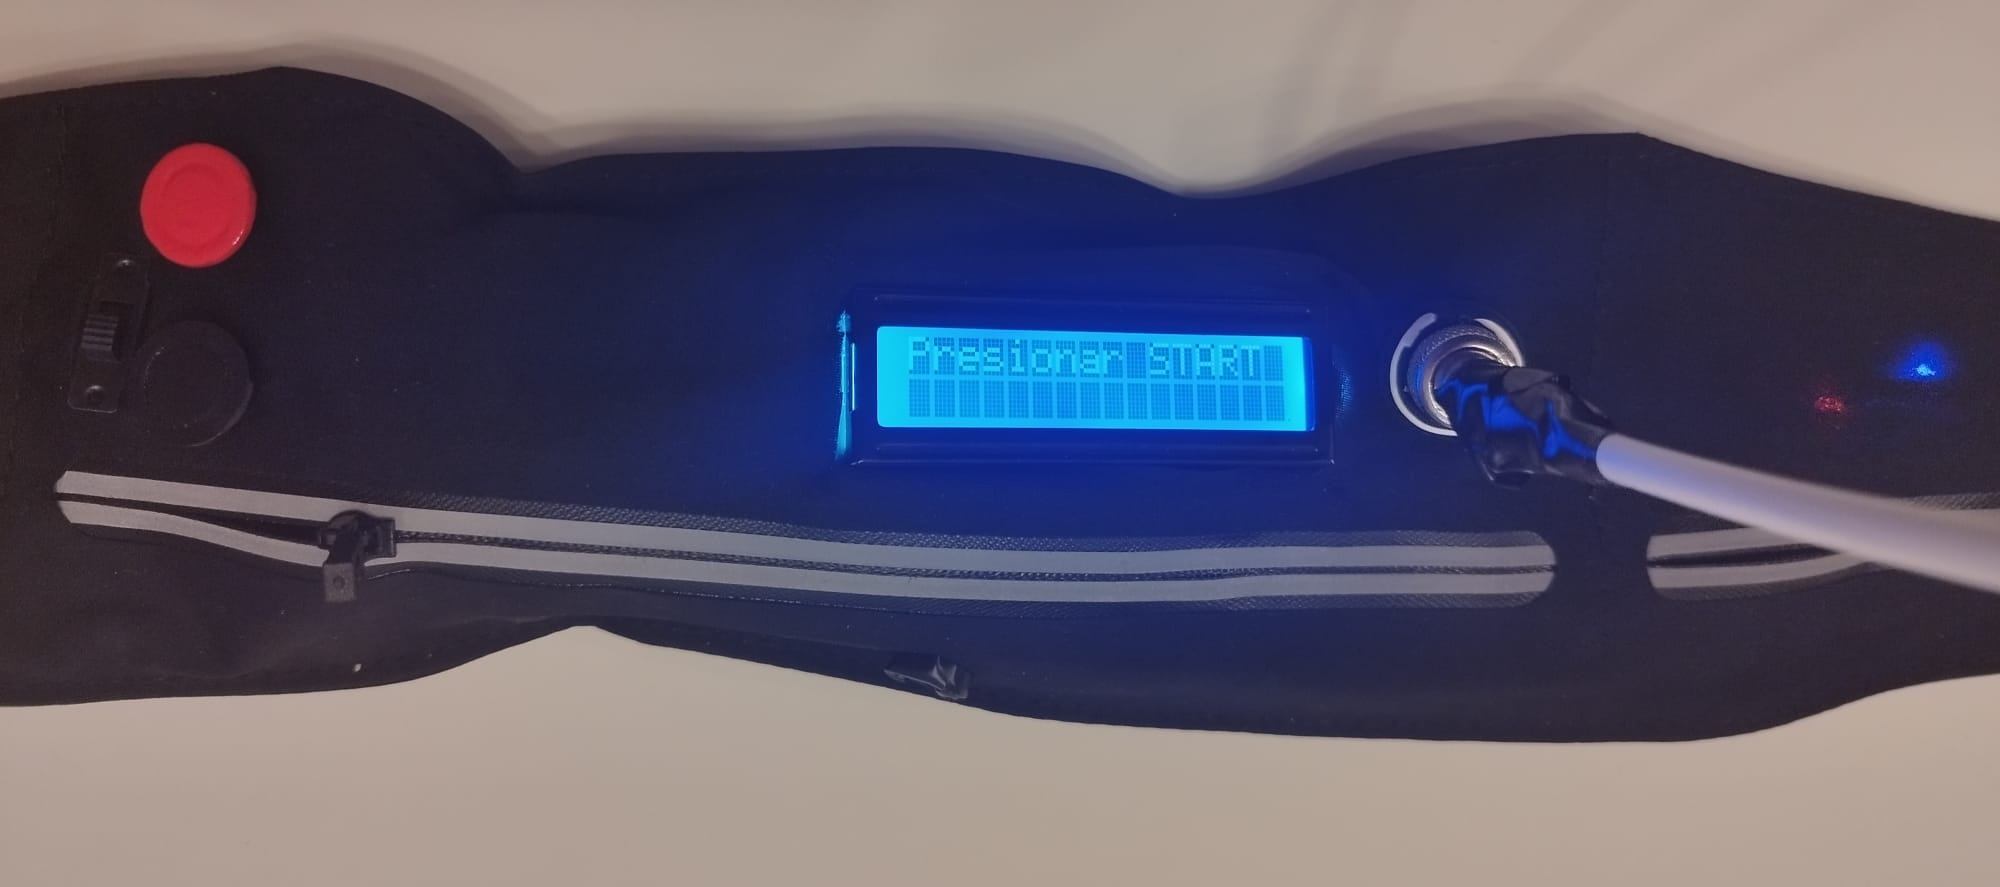
\includegraphics[width=1\textwidth]{img/prototipoencendido.jpg}
    \caption{Prototipo hardware encendido. Fuente propia.}
    \label{fig:prototipoencendido}
\end{figure}

Se alcanzaron los objetivos software relativos a la aplicación web: función de inserción de pautas de medicación para un paciente por parte de usuarios de tipo 'profesional', función web para los usuarios de tipo 'paciente' de registro de un diario de tomas de medicaciones y fluctuaciones motoras, prueba de personalización del número de segundos que el dispositivo detecta como congelamiento muscular, generación de gráficas a partir de los datos registrados y descarga de un informe relativo a las actividades registradas.

El script de Arduino fue editado satisfactoriamente, flexibilizando la detección de congelamientos de la marcha para tener en cuenta la prueba de personalización y controlando el encendido de módulo láser al detectar dichos congelamientos.

El objetivo relativo al almacenamiento de fecha y hora de cada actividad mediante implementación de un módulo de reloj RTC en el hardware fue alcanzado con un método distinto: almacenando la fecha y hora de guardado de cada actividad utilizando javascript, sin adición de módulos software adicionales.
\section{Discusión.}
Con el objetivo de contextualizar los resultados obtenidos durante el proyecto, se presenta una comparación de las características más relevantes de los mismos con los resultados otros trabajos.

En la tabla \ref{tab:comparacion1} se comparan las funciones de la solución tecnológica presentada en el artículo \cite{GONCALVES2021115653}, el cual ha sido previamente analizado en el apartado 'Conceptos teóricos' de este trabajo. Esta solución tecnológica ha sido escogida para realizar esta comparación debido a las inmensas similitudes en ambos proyectos: utilización de sensor inercial MPU-6050 para la monitorización de la marcha en pacientes con Párkinson, desarrollo de aplicación móvil conectada al hardware... 

% Please add the following required packages to your document preamble:
% \usepackage[table,xcdraw]{xcolor}
% Beamer presentation requires \usepackage{colortbl} instead of \usepackage[table,xcdraw]{xcolor}
\begin{table}[]
\begin{tabular}{l|
>{\columncolor[HTML]{FFFFFF}}l |
>{\columncolor[HTML]{FFFFFF}}l |}
\cline{2-3}
                                                                                                                                                                              & \cellcolor[HTML]{C0C0C0}Proyecto actual & \cellcolor[HTML]{C0C0C0}\begin{tabular}[c]{@{}l@{}}Sistema de \\monitorización\\ de la marcha\end{tabular} \\ \hline
\multicolumn{1}{|l|}{\cellcolor[HTML]{EFEFEF}\begin{tabular}[c]{@{}l@{}}Adquisición de datos \\ con MPU-6050\end{tabular}}                                                    & Sí                                      & Sí                                                                                                       \\ \hline
\multicolumn{1}{|l|}{\cellcolor[HTML]{EFEFEF}\begin{tabular}[c]{@{}l@{}}Unidad de almacenamiento \\ de datos (tarjeta SD)\end{tabular}}                                       & No                                      & Sí                                                                                                       \\ \hline
\multicolumn{1}{|l|}{\cellcolor[HTML]{EFEFEF}\begin{tabular}[c]{@{}l@{}}Comunicación bluetooth \\ con aplicación móvil\end{tabular}}                                          & Sí                                      & Sí                                                                                                       \\ \hline
\multicolumn{1}{|l|}{\cellcolor[HTML]{EFEFEF}\begin{tabular}[c]{@{}l@{}}Transmisión de los datos obtenidos\\  en tiempo real a la app\end{tabular}}                           & Sí                                      & Sí                                                                                                       \\ \hline
\multicolumn{1}{|l|}{\cellcolor[HTML]{EFEFEF}\begin{tabular}[c]{@{}l@{}}Integración de los datos con un \\ diario de síntomas del paciente\end{tabular}}                      & Sí                                      & No                                                                                                       \\ \hline
\multicolumn{1}{|l|}{\cellcolor[HTML]{EFEFEF}Generación de gráficas con los datos}                                                                                            & Sí (más básicas)                        & Sí                                                                                                       \\ \hline
\multicolumn{1}{|l|}{\cellcolor[HTML]{EFEFEF}Generación de informes pdf}                                                                                                      & Sí                                      & No                                                                                                       \\ \hline
\multicolumn{1}{|l|}{\cellcolor[HTML]{EFEFEF}\begin{tabular}[c]{@{}l@{}}Interfaz de escritorio en MATLAB para \\ el análisis detallado de los datos almacenados\end{tabular}} & No                                      & Sí                                                                                                       \\ \hline
\end{tabular}
\caption{Comparación entre el presente proyecto y un proyecto externo analizado previamente \cite{GONCALVES2021115653} }
\label{tab:comparacion1}
\end{table}

Teniendo en cuenta que el presente trabajo propone mejoras sobre un prototipo previamente construido a lo largo de los proyectos \cite{Gonzalez2023} \cite{Martos2024}  es importante diferenciar los aspectos del prototipo final que ya habían sido alcanzados en proyectos previos de las novedades. Esta diferencia puede observarse en la tabla \ref{tab:comparacion2}.
% Please add the following required packages to your document preamble:
% \usepackage[table,xcdraw]{xcolor}
% Beamer presentation requires \usepackage{colortbl} instead of \usepackage[table,xcdraw]{xcolor}
\begin{table}[]
\begin{tabular}{l|
>{\columncolor[HTML]{FFFFFF}}l |
>{\columncolor[HTML]{FFFFFF}}l |}
\cline{2-3}
                                                                                                                                                                                                 & \cellcolor[HTML]{C0C0C0}Proyecto actual & \cellcolor[HTML]{C0C0C0}Prototipos anteriores \\ \hline
\multicolumn{1}{|l|}{\cellcolor[HTML]{EFEFEF}\begin{tabular}[c]{@{}l@{}}Adquisición de datos \\ con MPU-6050\end{tabular}}                                                                       & Sí                                      & Sí                                            \\ \hline
\multicolumn{1}{|l|}{\cellcolor[HTML]{EFEFEF}\begin{tabular}[c]{@{}l@{}}Comunicación bluetooth \\ con aplicación móvil\end{tabular}}                                                             & Sí                                      & Sí                                            \\ \hline
\multicolumn{1}{|l|}{\cellcolor[HTML]{EFEFEF}\begin{tabular}[c]{@{}l@{}}Transmisión de los datos obtenidos\\  en tiempo real a la app\end{tabular}}                                              & Sí                                      & Sí                                            \\ \hline
\multicolumn{1}{|l|}{\cellcolor[HTML]{EFEFEF}\begin{tabular}[c]{@{}l@{}}Almacenamiento de los datos en base\\ de datos SQL\end{tabular}}                                                         & Sí                                      & Sí                                            \\ \hline
\multicolumn{1}{|l|}{\cellcolor[HTML]{EFEFEF}\begin{tabular}[c]{@{}l@{}}Recogida de datos diarios sobre\\ fluctuaciones motoras y tomas\\ de medicación\end{tabular}}                            & Sí                                      & No                                            \\ \hline
\multicolumn{1}{|l|}{\cellcolor[HTML]{EFEFEF}\begin{tabular}[c]{@{}l@{}}Integración de los datos con un \\ diario de síntomas del paciente\end{tabular}}                                         & Sí                                      & No                                            \\ \hline
\multicolumn{1}{|l|}{\cellcolor[HTML]{EFEFEF}Generación de gráficas con los datos}                                                                                                               & Sí (básicas)                            & No                                            \\ \hline
\multicolumn{1}{|l|}{\cellcolor[HTML]{EFEFEF}Generación de informes pdf}                                                                                                                         & Sí                                      & No                                            \\ \hline
\multicolumn{1}{|l|}{\cellcolor[HTML]{EFEFEF}\begin{tabular}[c]{@{}l@{}}Personalización del tiempo de reposo del \\ sensor MPU-6050 que se considera \\ congelamiento de la marcha\end{tabular}} & Sí                                      & No                                            \\ \hline
\end{tabular}
\caption{Comparación entre el presente proyecto y prototipos anteriores }
\label{tab:comparacion2}
\end{table}


\capitulo{6}{Conclusiones}
El desarrollo de este proyecto ha concluido con la presentación de una solución tecnológica hardware/software que cumple los principales objetivos propuestos. En este TFG se consiguen ampliar las funciones de la aplicación web, el script Arduino y el hardware utilizado, resultando en un prototipo más cómodo y útil a la hora de evaluar la progresión de la enfermedad de Párkinson.

Evolucionando algunos aspectos del prototipo propuesto, mencionados en el apartado de 'Líneas futuras', este prototipo podría empezar a probarse en pacientes con Párkinson para estudiar su posible uso regular, ya que resulta una herramienta muy útil, económica y sencilla de utilizar para las personas con Párkinson y los profesionales de la Salud que los tratan.

\section{Aspectos relevantes.}
A pesar del cumplimiento general de los requisitos observados, a lo largo del proyecto se realizaron una serie de cambios en los planteamientos relativos al desarrollo hardware y software:

Uno de los objetivos hardware propuestos en este trabajo era la inclusión del módulo RTC. Este módulo actúa como reloj, por lo cual se planteó como una opción viable para el almacenamiento de la fecha y hora de realización de actividades. Se realizaron pruebas utilizando este sensor en el script Arduino mediante varias bibliotecas específicas para este tipo de módulos. Sin embargo, los mejores resultados fueron la devolución de la fecha y hora de última compilación. Es decir, se consiguió que almacenase la fecha y hora del dispositivo desde el cual se cargaba el código pero no que dicha hora avanzase a partir de esta carga del script.

Durante estas complicaciones a la hora de insertar el RTC, surgió como idea alternativa el almacenamiento de fecha y hora de guardado de la actividad mediante javascript: Los datos de las actividades pasan por una serie de códigos en el backend de la aplicación, incluyendo como último paso el procesamiento de un servidor javascript (server.js) que se encarga de insertar los datos en la base de datos. En este script se incluyó el almacenamiento de fecha y hora, que junto al almacenamiento ya implementado de la duración de la actividad cubrían a la perfección las funciones que habían sido previamente planteadas para el módulo.

Al inicio del proyecto, se planteó la posibilidad de automatizar la calibración del sensor. Esta calibración, resultaba posible tan sólo al conectar mediante cable a un ordenador el prototipo, utilizando el script Arduino de calibración. Debido a la incomodidad derivada de la apertura del prototipo, conexión del mismo y cambio de scripts Arduino surgió la idea de una posible calibración automática llevada a cabo desde la app, incluyendo el script de calibración en el script general.

Sin embargo, tras probar el script de calibración e intentar brevemente su inclusión en el script general para poder utilizarlo sin cambiar códigos desde la página web se llegó a la conclusión de que esto no iba a resultar sencillo y no iba a aportar tanto valor al prototipo, ya que el script de calibración implementa una comunicación serial entre el dispositivo y dicho script que hace que la calibración resulte muy cómoda desde Arduino IDE, y que requeriría un cambio total y grandes complicaciones para cambiar esta comunicación serial y poder interactuar en la calibración desde la página web. Debido a esto, se decidió dejar de lado esta idea, centrando la atención en otros objetivos más relevantes.

Un último aspecto a destacar, es la ejecución de archivos python por parte de la página web para la generacion de gráficas: estos archivos devuelven satisfactoriamente las gráficas requeridas, actualizando con cada ejecución los datos cuando son ejecutados de forma individual en Visual Studio. Las gráficas creadas se almacenan en el mismo directorio donde se encuentran los archivos de código. 

Sin embargo, cuando se intentan ejecutar los archivos python de generación de gráficas desde la página web, de forma previa a la visualización de las mismas, en ocasiones no se actualizan los datos de las gráficas automáticamente, y sencillamente se muestran las imágenes guardadas por última vez en el directorio correspondiente. Esto hace recomendable la ejecución temporal de los archivos python desde Visual Studio, con el objetivo de mostrar datos actualizados en las estadísticas.






\capitulo{7}{Lineas de trabajo futuras}

En este proyecto se concluye la creación de un prototipo hardware/software para la monitorización de párkinson desarrollado a partir de los trabajos \cite{Gonzalez2023} 
 \cite{Martos2024}, añadiendo funciones como la personalización del tiempo registrado como congelación de la marcha, el registro de un diario de tomas y fluctuaciones, la visualización de gráficas y descarga de informes a partir de las actividades registradas... Se obtuvo un hardware que proporciona más comodidad al usuario y una respuesta en tiempo real a las situaciones de cese de la marcha.\\

Para la mejora de este prototipo se propone una edición del código Arduino que permita utilizar de forma más amplia las funcionalidades del sensor MPU-6050. De esta forma, se podrían detectar movimientos irregulares en la marcha causados por bloqueos de la marcha que no necesariamente desembocan en cese de la marcha (bloqueos parciales/bloqueos transitorios).\\

Teniendo esta capacidad podrían incluso llegar a distinguirse ceses voluntarios e involuntarios de la marcha, ya que los ceses involuntarios presentarán previos movimientos irregulares en la marcha. Esta distinción puede aportar un gran avance en la facilidad de uso del prototipo, pudiendo descartar los botones de start y stop, ya que el programa podría desactivarse de manera automática ante un cese voluntario de la marcha. Esto permitiría registrar actividades de duración más larga, pulsando tan sólo el botón ON-OFF al inicio y fin de las mismas.\\

La precisión de las medidas recogidas por el sensor MPU-6050 podría aumentarse utilizando 2 sensores en la tobillera: de esta forma, en caso de registrar valores similares podría hacerse la media de estos, aportando una mayor fiabilidad o en caso de registrar valores muy distintos podría saltar un indicador de la necesidad de recalibrar ambos sensores.\\

La inclusión de una tarjeta SD en el dispositivo resultaría interesante, permitiendo guardar los datos sin necesidad de que el dispositivo esté conectado mediante bluetooth a un ordenador o teléfono móvil. Los datos almacenados en la tarjeta SD podrían descargarse periódicamente para insertarlos en la app y asegurar su utilización.\\

Un avance que mejoraría de forma significativa la comodidad de uso del prototipo pero que resulta complicada en su implementación es la eliminación del cable que conecta el cinturón con la tobillera, implementando una comunicación inalámbrica entre ambas partes. Esto implicaría además del uso de comunicación inalámbrica por bluetooth/WiFi/radio frecuencia la adición de un microcontrolador adicional en la tobillera, como podría ser el Arduino Nano, lo cual requeriría también otra fuente de alimentación.\\




\bibliographystyle{apalike}


\printbibliography
\end{document}
